%class
	\documentclass{beamer}

%template
	\usetheme{HannoverSalman}
	\setbeamertemplate{navigation symbols}{}
	%\setbeamertemplate{footline}{\centering{\insertframenumber/\insertpresentationendpage}}
	%\setbeamertemplate{footline}{\hspace*{.5cm}\scriptsize{\hfill\insertframenumber\hspace*{.5cm}}} 


%packages
	\usepackage{amsmath, amssymb, graphicx,cancel}
	\usepackage[absolute,overlay]{textpos}
	\usepackage{subfigure}
	\usepackage{caption}\captionsetup{labelformat=empty,labelsep=none}
	\usepackage{geometry}
	\geometry{verbose}
	\usepackage{color}
	\usepackage{xmpmulti}
	\usepackage[3D]{movie15}
	\usepackage{hyperref}
%	\usepackage{bookmark}
	\usepackage[open,openlevel=4,atend]{bookmark}
	%\bookmarksetup{color=blue}
	\usepackage{multirow}
	\usepackage[style=numeric,defernumbers, authoryear]{biblatex}
	%\usepackage[square,sort]{natbib}
	%\usepackage{fancyhdr}%\pagestyle{fancy} 

	
	\hypersetup{bookmarksdepth = 4}


%citations files
	\bibliography{MyCitations}

%logoCSIPCPL
    \setlength{\TPHorizModule}{1mm}
    \setlength{\TPVertModule}{1mm}
    \newcommand{\logoCSIPCPL}
    {
    	\begin{textblock}{1}(100,2) %(100,85)  for bottom
    		
\includegraphics[width=1.5cm]{figs/logo_CSIP}
    	\end{textblock}
    	
	\begin{textblock}{1}(117,1) %(117,85)  for bottom
    		
\includegraphics[width=1.0cm]{figs/logo_CPL}
    	\end{textblock} 
    }

%logo evolution
    \newcommand{\logoEvolution}
    {    	
	\begin{textblock}{1}(110,1) %(117,85)  for bottom
    		\includegraphics[width=0.65in]{figs/logo_evolution.pdf}
    	\end{textblock} 
    }

%logo Qualcomm
    \newcommand{\logoQualcomm}
    {
    	\begin{textblock}{1}(110,2) %(100,85)  for bottom
    		\includegraphics[width=1.5cm]{figs/logo_qualcomm.jpg}
    	\end{textblock}
    }
%logo Qualcomm (long)
    \newcommand{\logoQualcommllong}
    {
    	\begin{textblock}{1}(0,0) 
    		\includegraphics[width=1.25in]{figs/logo_qualcomm_long.jpg}
    	\end{textblock}
    }

%logo Tech Tower
    \newcommand{\logoTechTower}
    {
    	\begin{textblock}{1}(0,0) 
    		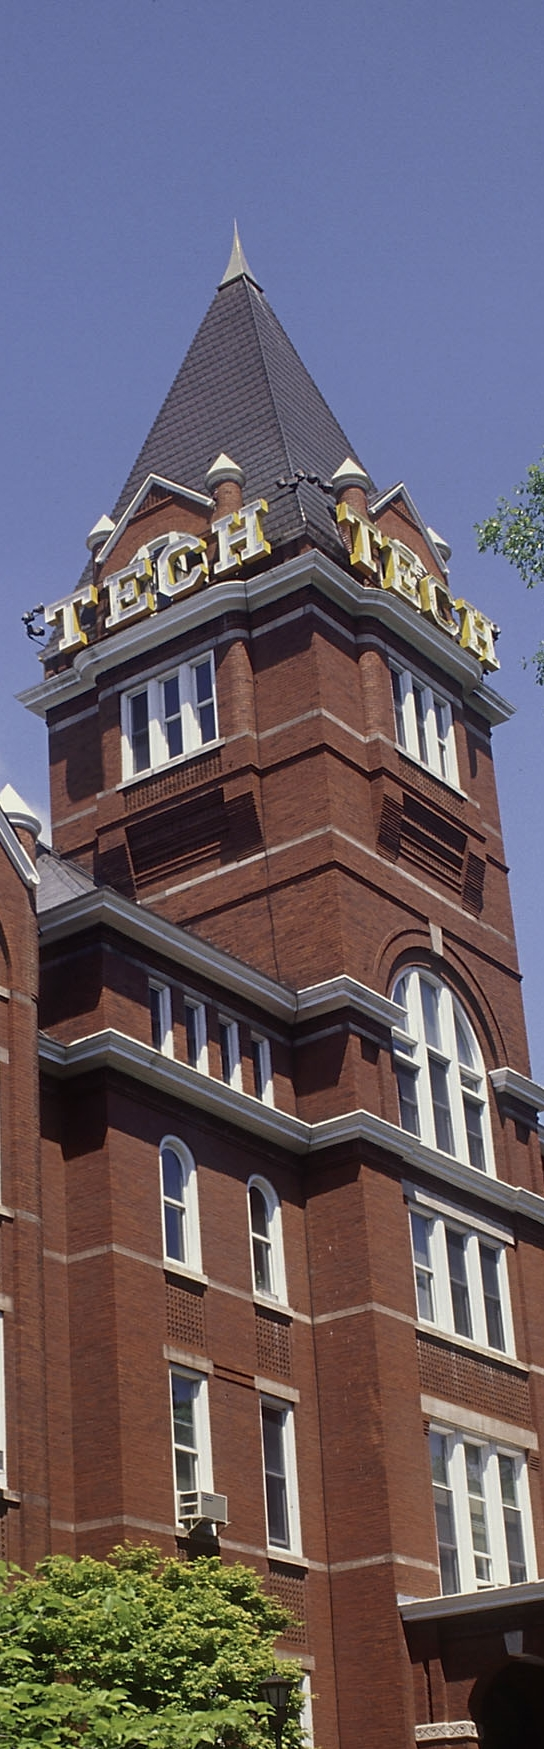
\includegraphics[width=1.25in]{figs/logo_TechTower.jpg}
    	\end{textblock}
    }

%logo tree
    \newcommand{\logoTree}
    {
    	\begin{textblock}{1}(0,0) 
    		\includegraphics[width=1.25in]{figs/logo_tree.jpg}
    	\end{textblock}
    }
%page numbers
    \newcommand{\mypagenum}
    {
    	\begin{textblock}{1}(1,94) 
		{\tiny \color[rgb]{0.2,0.2,1}\insertframenumber} %\insertframenumber,\insertpresentationendpage, \inserttotalframenumber
    	\end{textblock}
    }
%my footnote citation
	\newcommand{\myFootnoteCitation}[2]
	{
		\footnote{\tiny \citeauthor{#1}, \emph{#2}, \citeyear{#1}.}  %\citeauthor{#1}, \citetitle{#1}, #2 \citeyear{#1}.
	}
%my refer to citation
	\newcommand{\mycite}[1]
	{
		\emph{\citeauthor{#1} (\citeyear{#1})}
	}
%my footnote website citation
	\newcommand{\myFootnoteWebsiteCitation}[1]
	{
		\footnote{\tiny \citeauthor{#1}}
	}

\let\thefootnote\relax\footnotetext{Footnotetext without footnote mark}


%section underline
%\newcommand{\tmpsection}[1]{}
%\let\tmpsection=\section
%\renewcommand{\section}[1]{\tmpsection{\underline{#1}}}



%commands
	\newcommand{\likelihood}{p(Z_k| x_k) }						%likelihood
	\newcommand{\prior}{p(x_k)  } 								%prior
	\newcommand{\posterior} {p(x_k| Z_k)}						%posterior
	\newcommand{\prediction} {p(x_k| Z_{k-1})}					%prediction
	\newcommand{\update} {p(x_k|Z_k)}							%update
	\newcommand{\observations} {p(Z_k)}						%observations
	\newcommand{\prevobservations} {p(Z_{k-1})}				%previous observations
	\newcommand{\dxpk} {dx_{k-1}}							%dx_{k-1}
	\newcommand{\ChapKolm}{\int{p(x_k| x_{k-1})p(x_{k-1}|Z_{k-1})} \dxpk} %Chapman Kolmogorov

	%algorithm specific: JPDAF
	\newcommand{\likelihoodJPDAF}{p(Z_k| \chi, m, Z_{k-1}) }		%1. likelihood
	\newcommand{\priorJPDAF}{p(\chi|m, Z^{k-1}} 				%2. prior	
	\newcommand{\observationsJPDAF} {p(Z_k}					%3. observations
	\newcommand{\posteriorJPDAF} {p(\chi| Z_k)}					%4. posterior

%environments
	\newenvironment{changemargin}[2]
	{
	  	\begin{list}{}
		{
			\setlength{\topsep}{0pt}%
			\setlength{\leftmargin}{#1}%
			\setlength{\rightmargin}{#2}%
			\setlength{\listparindent}{\parindent}%
			\setlength{\itemindent}{\parindent}%
			\setlength{\parsep}{\parskip}%
		}
	  	\item[]
		}
		{\end{list}
	}
%figures

%colors
\definecolor{darkgreen}{rgb}{0,0.5,0}

%personal details
	\author{Salman Aslam}
	\institute{Advisor, Dr Christopher Barnes (ECE)\\Co-advisor, Dr Aaron Bobick (CoC)\\Georgia Institute of Technology}
	\date{}

\begin{document}
\definecolor{darkgreen}{rgb}{0,0.5,0}
\newcommand{\Ntrg}{\big[N_{t=1, m=1} + \lambda \big] + \big[N_{t=1, m=2} + \lambda \big] + \ldots + \big[N_{t=1, m=M} + \lambda \big]}
\newcommand{\jointcnt}{\sum\limits_{n_{trg}=1}^{N_{trg}}I(X_t=x_t, X_{t-1}=x_{t-1})}
\newcommand{\singlecnt}{\sum\limits_{n_{trg}=1}^{N_{trg}}I(X_{t-1}=x_{t-1})}
\newcommand{\singlep}{p(X_{t-1}=x_{t-1})}
\newcommand{\singlepone}{p(X_{t-1}=1)}
\newcommand{\singleptwo}{p(X_{t-1}=2)}
\newcommand{\singlepM}{p(X_{t-1}=M)}
\newcommand{\condp}{p(X_t=x_t | X_{t-1}=x_{t-1})}
\newcommand{\jointp}{p(X_t=x_t, X_{t-1}=x_{t-1})}
\newcommand{\KmeansOuterSum}{\sum\limits_{k=1}^K}
\newcommand{\KmeansInnerSum}{\sum\limits_{{i=1 \atop x_i \in \mathcal{K}_k}}^N}
\newcommand{\KmeansSum}{\KmeansOuterSum \KmeansInnerSum}
\newcommand{\RVQInnerSum}{\sum\limits_{{i=1 \atop g_i \mapsto m_{\tau, s}}}^N}
\newcommand{\RVQOuterSum}{\sum_{s=1}^S}
\newcommand{\RVQsum}{\KmeansOuterSum \sum\limits_{{i=1 \atop g_i \in \mathcal{K}_k}}^N}
\newcommand{\KmeansInner}{{(x_i - \mu_k)}^2}
\newcommand{\RVQinner}{            {(x_i  - \hat{\mu}^{(k)})}^2}
\newcommand{\RVQinneralternate}{{(g_i - m_\tau^{(k)})}^2}
\newcommand{\RVQinneralternatealternate}{{(g_i - m_{\tau, s})}^2}
\newcommand{\KmeansError}{\KmeansSum \KmeansInner}
\newcommand{\RVQerror}     {\KmeansSum \RVQinner}
\newcommand{\RVQerroralternate}{\RVQsum \RVQinneralternate}
\newcommand{\RVQunit}{x_i -\bigg(\sum_{t=1}^Tm^{(k)}_t\bigg)}
\newcommand{\RVQequivalentCodevector}{\sum_{t=1 }^Tm^{(k)}_t}
\newcommand{\RVQequivalentCodevectorBroken}{\sum_{t=1 \atop t \neq \tau}^Tm^{(k)}_t+ m^{(k)}_\tau}
\newcommand{\RVQmultipleKmeans}{x_i -\bigg(\RVQequivalentCodevectorBroken\bigg)}
\newcommand{\RVQmultipleKmeansone}{x_i -\sum_{t=2}^Tm^{(k)}_t+ m^{(k)}_1\bigg)}
\newcommand{\RVQmultipleKmeansonealternate}{\bigg(x_i -\sum_{t=1 \atop t \neq \tau}^Tm^{(k)}_t\bigg) - m^{(k)}_\tau}
\newcommand{\RVQmultipleKmeanstwo}{x_i -\bigg(\sum_{t=1 \atop t \neq 2}^Tm^{(k)}_t+ m^{(k)}_2\bigg)}
\newcommand{\RVQmultipleKmeansT}{x_i -\bigg(\sum_{t=1}^{T-1}m^{(k)}_t+ m^{(k)}_2\bigg)}
\newcommand{\EucMatrix}
{
\left[
\begin{array}{lll}
r_{11} & r_{12} & t_x \\ 
r_{21} & r_{22} & t_y \\ 
0 & 0 & 1 \\ 
\end{array}
\right]
}	

\newcommand{\SimMatrix}
{
\left[
\begin{array}{lll}
sr_{11} & sr_{12} & t_x \\ 
sr_{21} & sr_{22} & t_y \\
0 & 0 & 1 \\ 
\end{array}
\right]
}

\newcommand{\AffMatrix}
{
\left[
\begin{array}{lll}
a &b & t_x \\ 
c & d & t_y \\
0 & 0 & 1 \\
\end{array}
\right]
}

\newcommand{\ProjMatrix}
{
\left[
\begin{array}{lll}
h_{11} & h_{12} & h_{13} \\ 
h_{21} & h_{22} & h_{23} \\ 
h_{31} & h_{32} & h_{33} \\ 
\end{array}
\right]
}

\newcommand{\RotMatrixTheta}
{
\left[
\begin{array}{rr}
\cos(\theta) & -\sin(\theta) \\ 
\sin(\theta) & \cos(\theta) \\ 
\end{array}
\right]
}

\newcommand{\RotMatrixPhi}
{
\left[
\begin{array}{rr}
\cos(\phi) & -\sin(\phi) \\ 
\sin(\phi) & \cos(\phi) \\ 
\end{array}
\right]
}

\newcommand{\RotMatrixminusPhi}
{
\left[
\begin{array}{rr}
\cos(-\phi) & -\sin(-\phi) \\ 
\sin(-\phi) & \cos(-\phi) \\ 
\end{array}
\right]
}


\newcommand{\EigenvalueMatrix}
{
\left[
\begin{array}{cc}
\lambda_1 & 0\\
0 & \lambda_2
\end{array}
\right]
}

\newcommand{\bigMatrix}
{
s \left[
\begin{array}{cc}
 (r)(a) + b &  (r)(d) - c \\
 (r)(c) - d &  (r)(b) + a
\end{array}
\right]
}


\newcommand{\bigMatrixTwo}
{
\left[
\begin{array}{cc}
(\lambda_2) p + (\lambda_1) q & (\lambda_2) s  - (\lambda_1) r \\
(\lambda_2) r  - (\lambda_1) s & (\lambda_2) q + (\lambda_1) p
\end{array}
\right]
}
\newcommand{\dr}{(\mathbf{x}_i-\boldsymbol\mu_k)^T(\mathbf{x}_i-\boldsymbol\mu_k) + \lambda({Q_{\textrm{max}}-Q_i})}

%####################################################################################################
\title{Target Tracking \\ Using \\Residual Vector Quantization}
%####################################################################################################
\begin{frame}[plain]\logoCSIPCPL\logoTechTower
	\titlepage
\end{frame}

\begin{frame}
\frametitle{Outline}
\logoCSIPCPL\logoTechTower
	\setcounter{tocdepth}{1}	
	\tableofcontents
\end{frame}

%####################################################################################################
\section{I. Background}
%####################################################################################################
\begin{frame}
\frametitle{Background}
\framesubtitle{}
\logoCSIPCPL\mypagenum
\vspace{0.2in}
\begin{itemize}
\item 2005: Dr Altunbasak, hierarchical motion vector estimation, background modeling
\item {\color{blue}Interest}: pattern recognition, signal processing
\item 2007: switched to Dr Bobick, robust computer vision on compressed video
\item 2010: Dr Barnes + Dr Bobick, RVQ as a pattern recognition method extended to several images
\end{itemize}
\begin{figure}
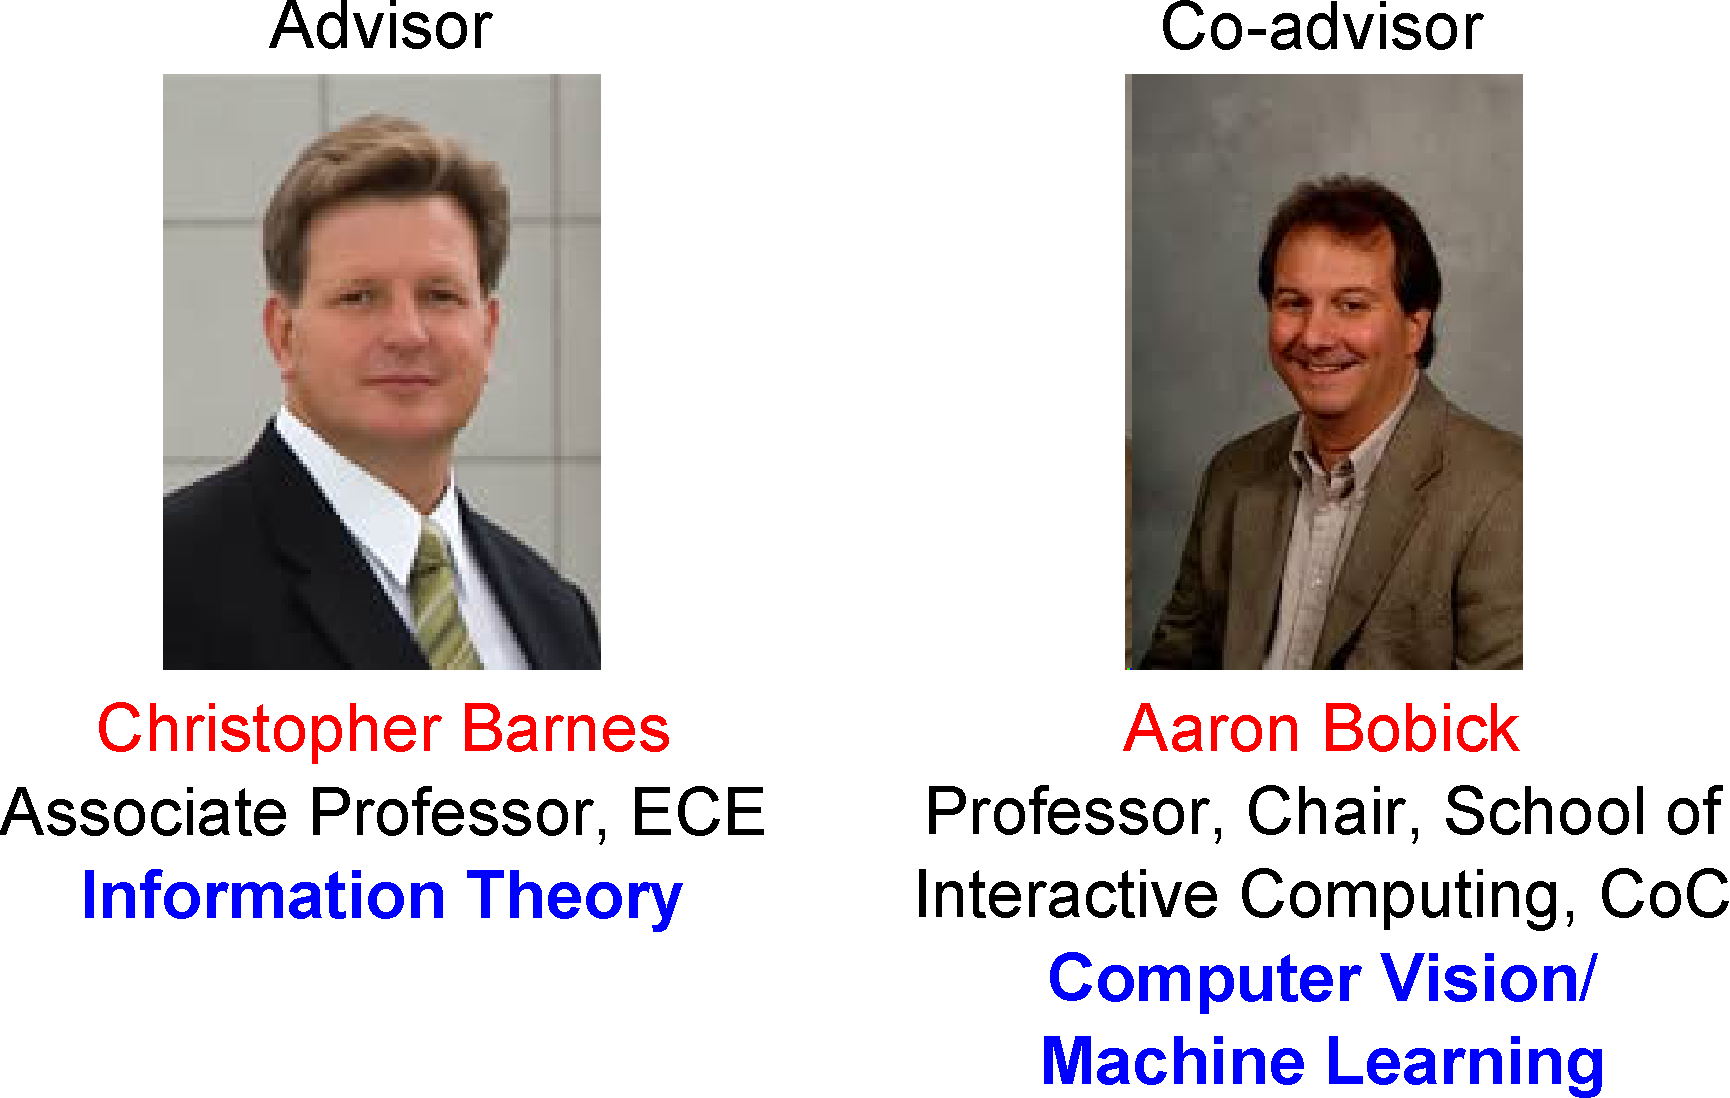
\includegraphics[width=0.73\textwidth]{thesis/professors.pdf}
\end{figure}
\end{frame}


\begin{frame}
\frametitle{Background}
\framesubtitle{}
\logoCSIPCPL\mypagenum
\begin{figure}[t]
\centering
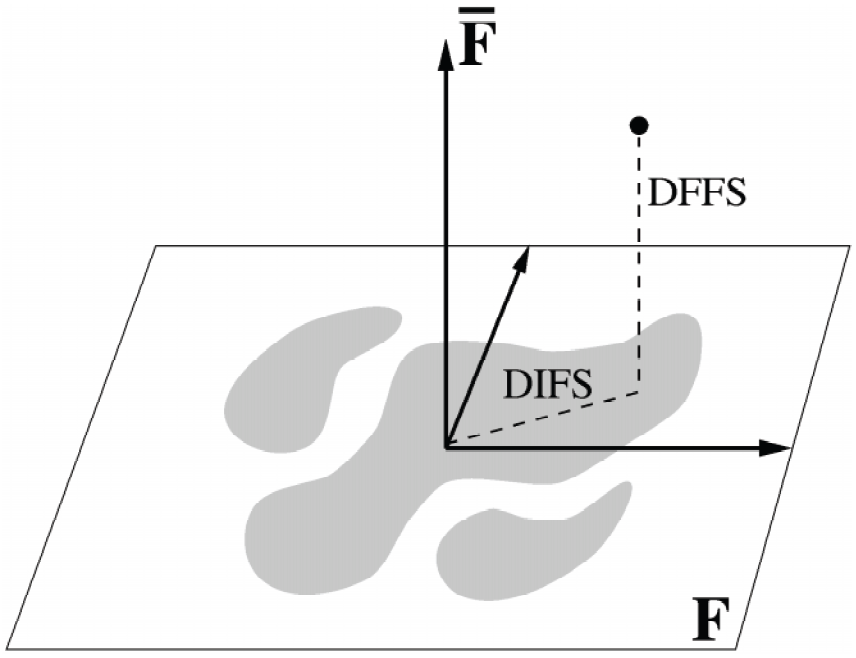
\includegraphics[width=0.5\textwidth]{thesis/1998_JNL_ProbVisLearning_Moghaddam_fig3.png}
\caption{Graphical illustration of DFFS (distance-from-feature-space) and DIFS (distance-in-feature-space).  The feature space is $\mathbf{F}$ while the subspace orthogonal to the feature space is $\bar{\mathbf{F}}$.  DFFS is the signal residual error and DIFS is the $\mathbf{F}$-space likelihood \cite{1997_JNL_EigenTRK_Moghaddam}.}
\label{fig:1997_JNL_DIFSDFFS_Moghaddam}
\end{figure}
\end{frame}

%==================================
\section{II. Tracking}
%==================================
%---------------------------------------------------------
\subsection{(a) Overview}
%---------------------------------------------------------
\begin{frame}
\frametitle{Tracking}
\framesubtitle{definition}
\logoCSIPCPL\mypagenum
	Estimate and maintain {\color{red}target state} over {\color{red}time}
	\begin{figure}
		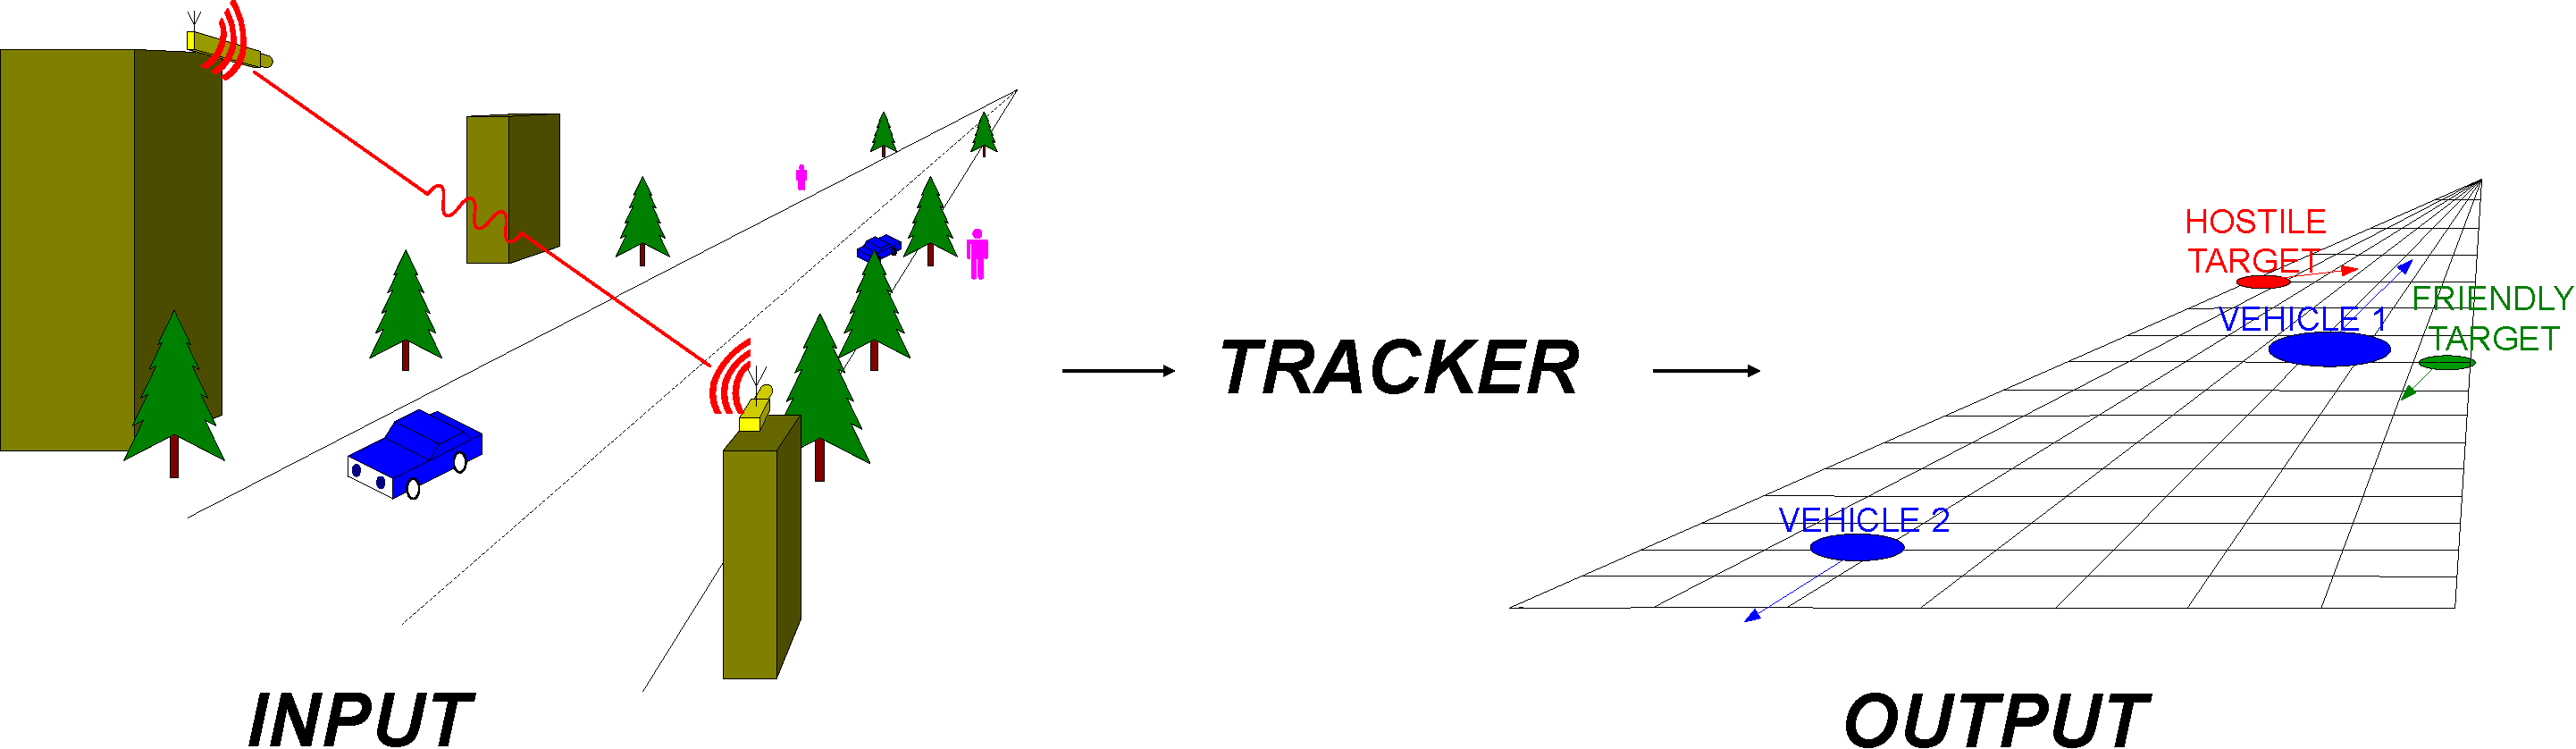
\includegraphics[width=1.0\textwidth]{thesis/TRK_overviewDiagram.pdf}
	\end{figure}
\end{frame}


\begin{frame}[plain]
\frametitle{Tracking}
\framesubtitle{overview\tiny{\footnote {Yilmaz et.al., 2006}}}
\logoCSIPCPL\mypagenum
	\begin{changemargin}{-1.3in}{0in}
		\begin{figure}
			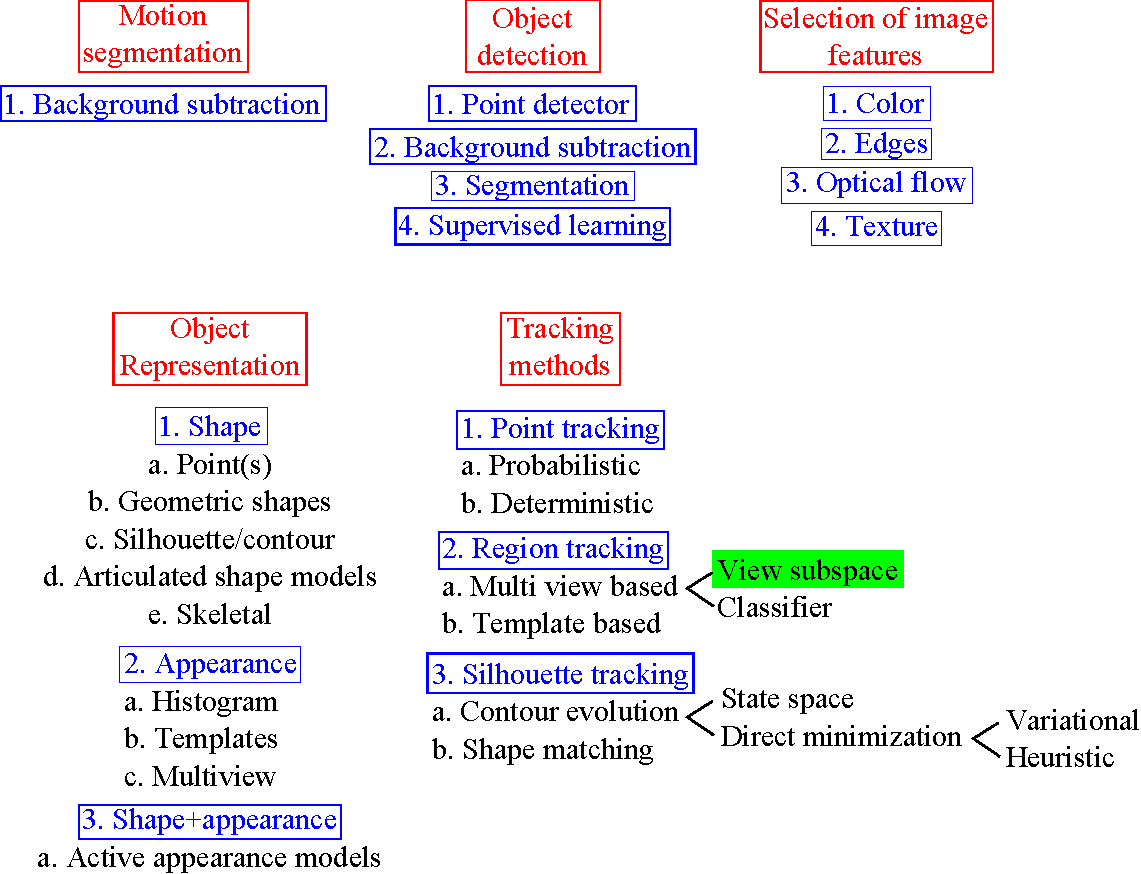
\includegraphics[width=1.3\textwidth]{thesis/TRK_overview.pdf}
		\end{figure}	
	\end{changemargin}
	\begin{block}{Tracking methods}
		\begin{itemize}
			\item Point
			\item Region
			\item Contour
		\end{itemize}
	\end{block}
\end{frame}



\begin{frame}
\frametitle{Tracking}
\framesubtitle{big picture}
\logoCSIPCPL\mypagenum
	\begin{figure}
		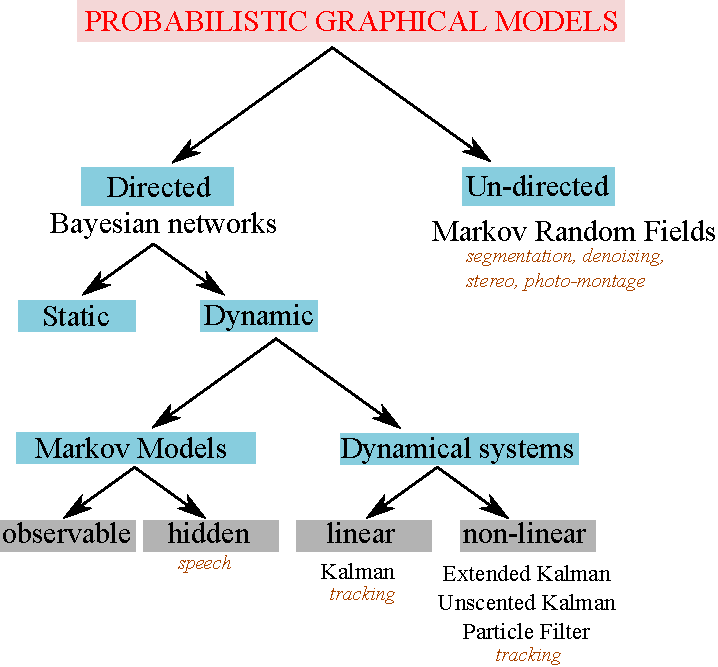
\includegraphics[width=0.9\textwidth]{thesis/PRML_PGM_overview.pdf}
	\end{figure}
\end{frame}





\begin{frame}
\frametitle{Tracking}
\framesubtitle{relationship with HMM}
\logoCSIPCPL\mypagenum
	\begin{figure}
		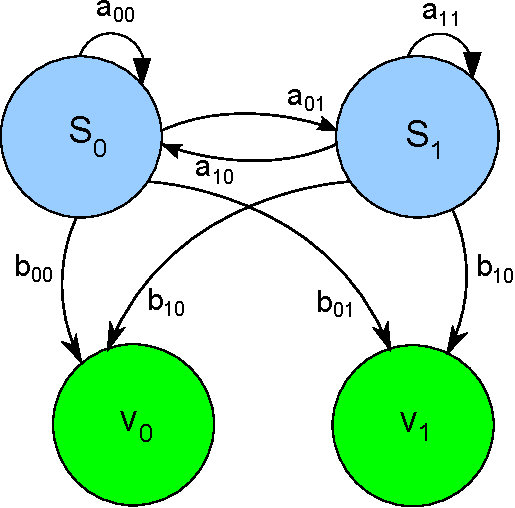
\includegraphics[height=0.3\textheight]{thesis/HMM_flowDiagram.pdf}
	\end{figure}
	\begin{figure}
		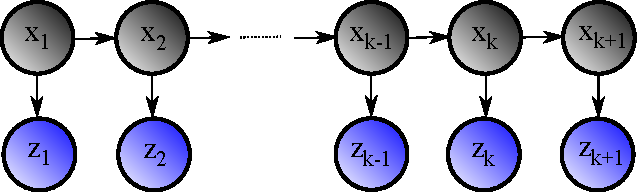
\includegraphics[width=1.0\textwidth]{thesis/HMM_flowDiagram2.pdf}
	\end{figure}
\end{frame}

\begin{frame}
\frametitle{Tracking}
\framesubtitle{update}
\logoCSIPCPL\mypagenum
	\begin{figure}
		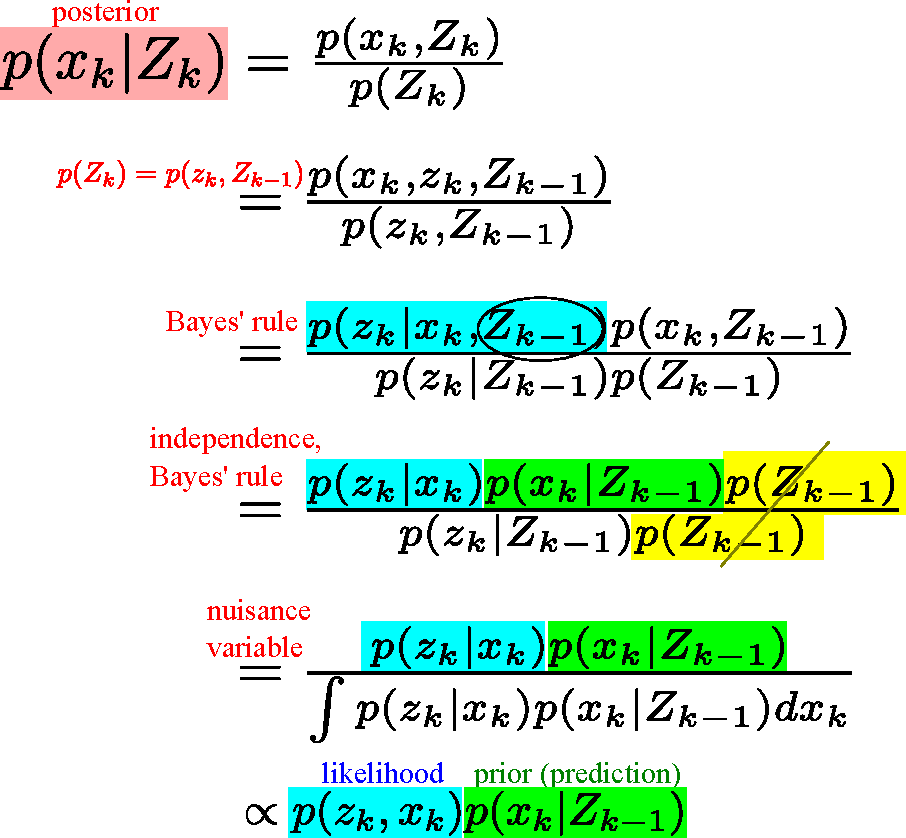
\includegraphics[width=1.0\textwidth]{thesis/TRK_EQN_update.pdf}
	\end{figure}
\end{frame}



\begin{frame}
\frametitle{Tracking}
\framesubtitle{prediction}
\logoCSIPCPL\mypagenum
	Chapman Kolmogorov equation
	\begin{figure}
		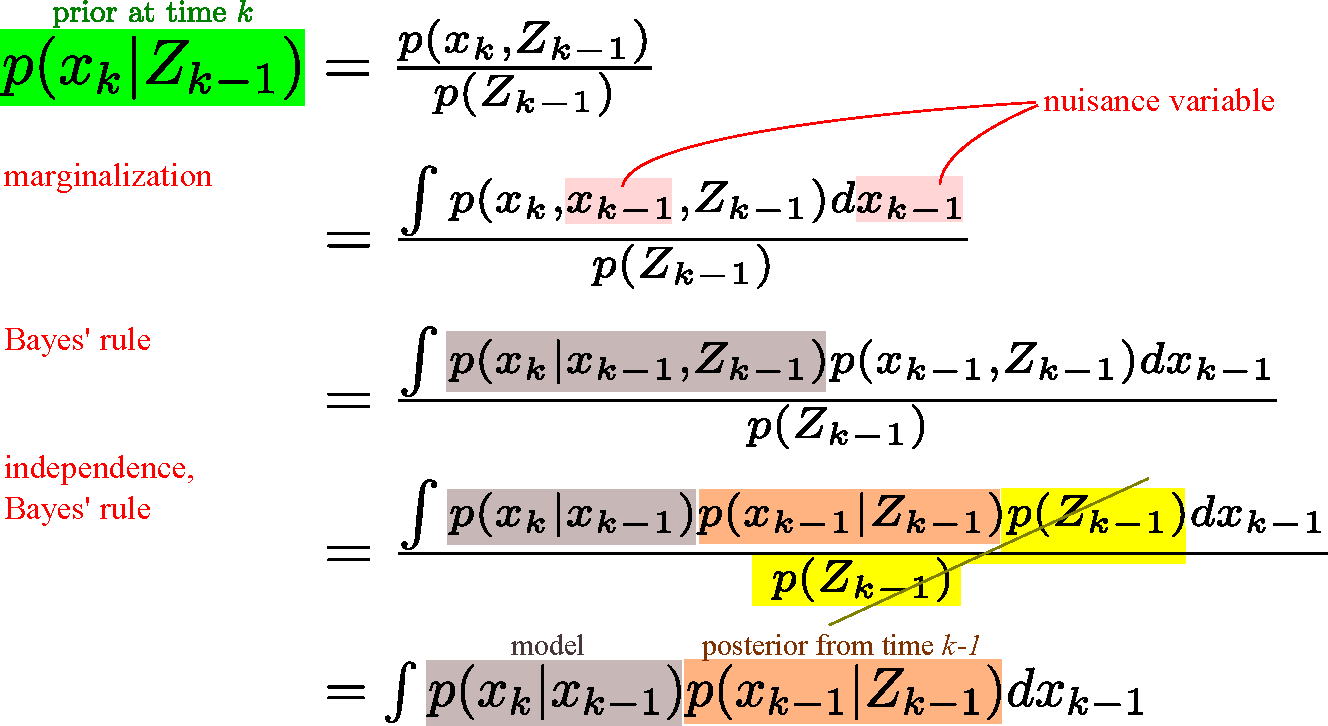
\includegraphics[width=1.0\textwidth]{thesis/TRK_EQN_prediction.pdf}
	\end{figure}
\end{frame}

%---------------------------------------------------------
\subsection{(b) Radars}
%---------------------------------------------------------
\begin{frame}
\frametitle{Originally: radars}
\framesubtitle{Kalman Filter}
\logoCSIPCPL\mypagenum
\begin{figure}
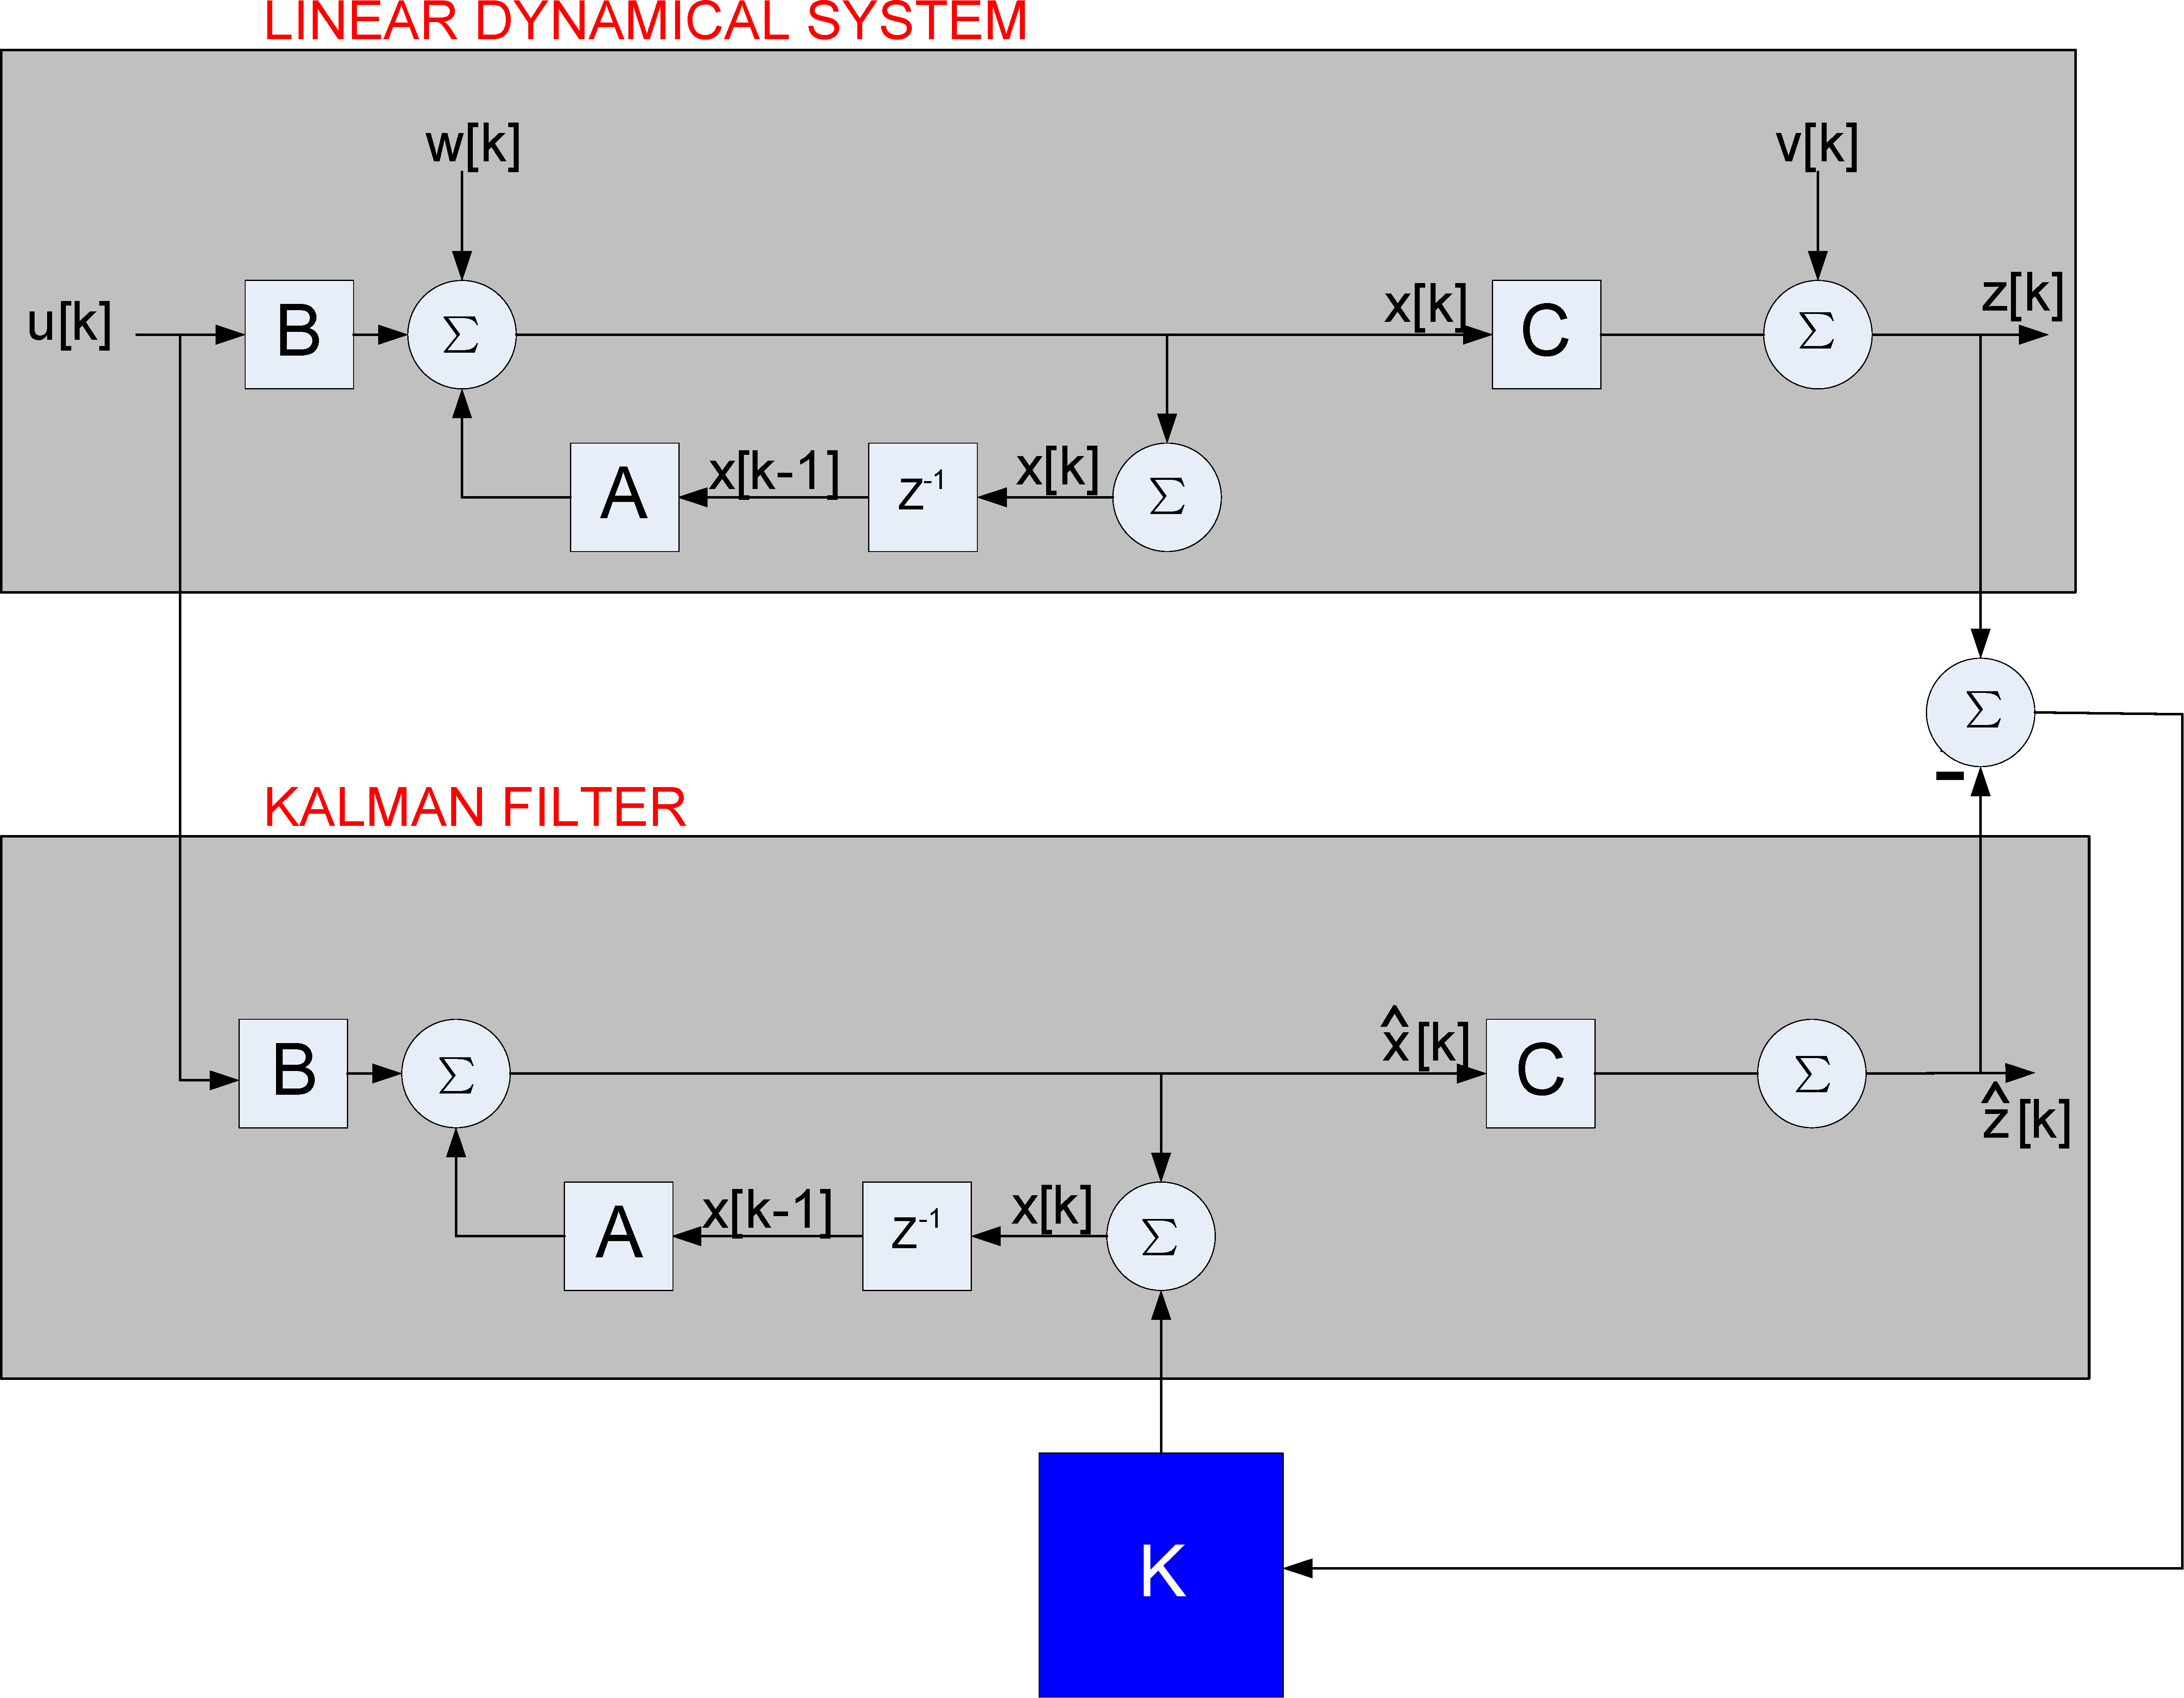
\includegraphics[width=1.0\textwidth]{thesis/TRK_KalmanFilter_blockDiagram.pdf}
\end{figure}
\end{frame}



\begin{frame}
\frametitle{Radar tracking\footnote{Bar-Shalom et al., 2009}}
\framesubtitle{}
\logoCSIPCPL\mypagenum
\setcounter{subfigure}{0}
\begin{figure}
\subfigure[US Navy, long-range surveillance]{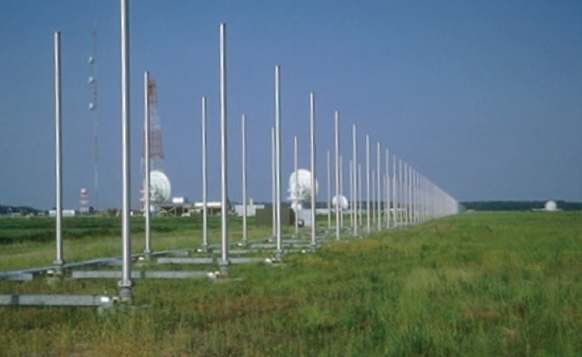
\includegraphics[height=0.2\textheight]{figs/TRK_PDAF_example_US_Navy_ROTHR.jpg}}\hspace{0.2in}
\subfigure[Theater High Altitude Area Defense]{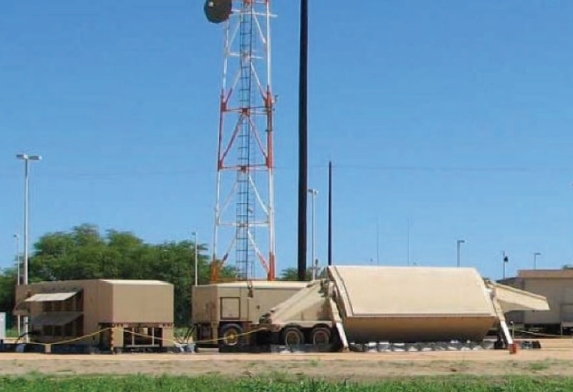
\includegraphics[height=0.2\textheight]{figs/TRK_JPDAF_example_THAAD.jpg}}
\subfigure[long-range surveillance against ICBMs]{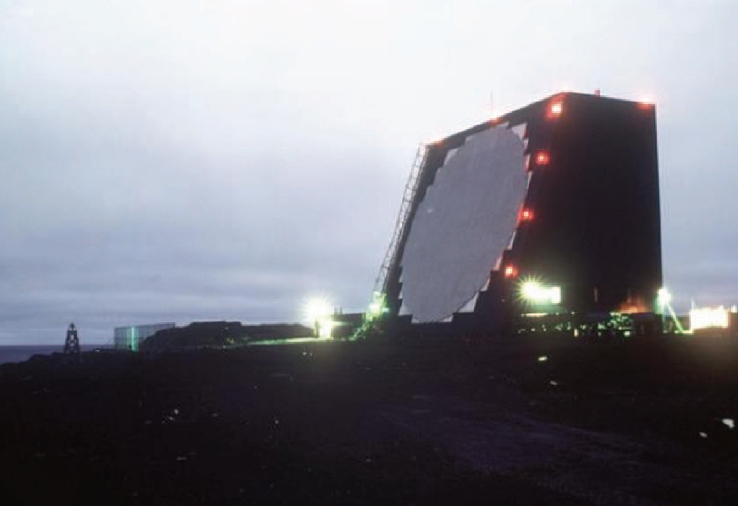
\includegraphics[height=0.2\textheight]{figs/TRK_JPDAF_example_Cobra.jpg}}\hspace{0.2in}
\subfigure[long-range surveillance against ICBMs]{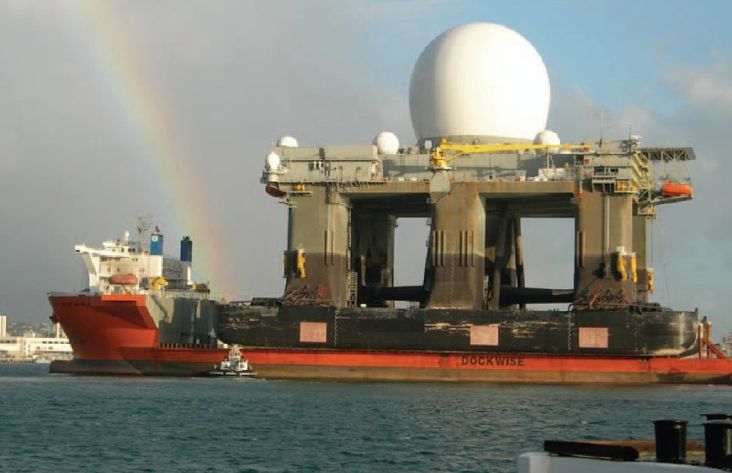
\includegraphics[height=0.2\textheight]{figs/TRK_JPDAF_example_SBX.jpg}}
\end{figure}
\end{frame}



\begin{frame}
\frametitle{Particle Filter}
\framesubtitle{multi-modal PDF}
\logoCSIPCPL\mypagenum
	\begin{figure}
		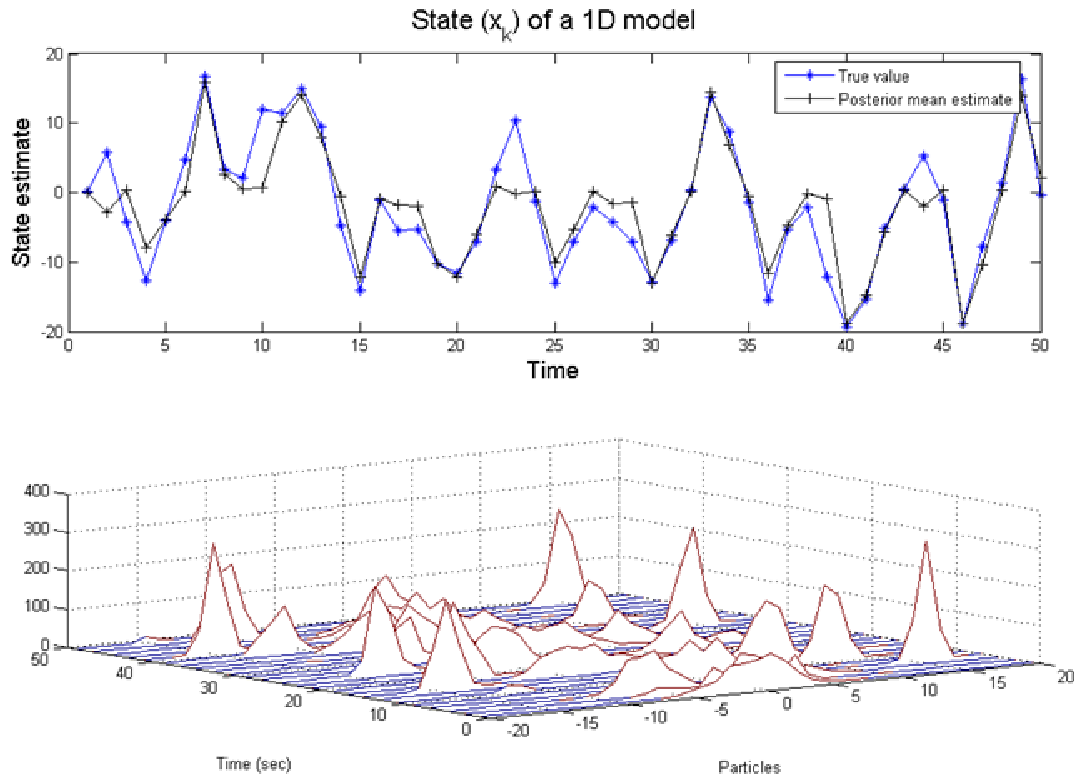
\includegraphics[width=1.0\textwidth]{thesis/TRK_ParticleFilter_multimodalPDF.pdf}
	\end{figure}	
\end{frame}


\begin{frame}
\frametitle{Tracking}
\framesubtitle{definition}
\logoCSIPCPL\mypagenum
\begin{figure}[t]
\center
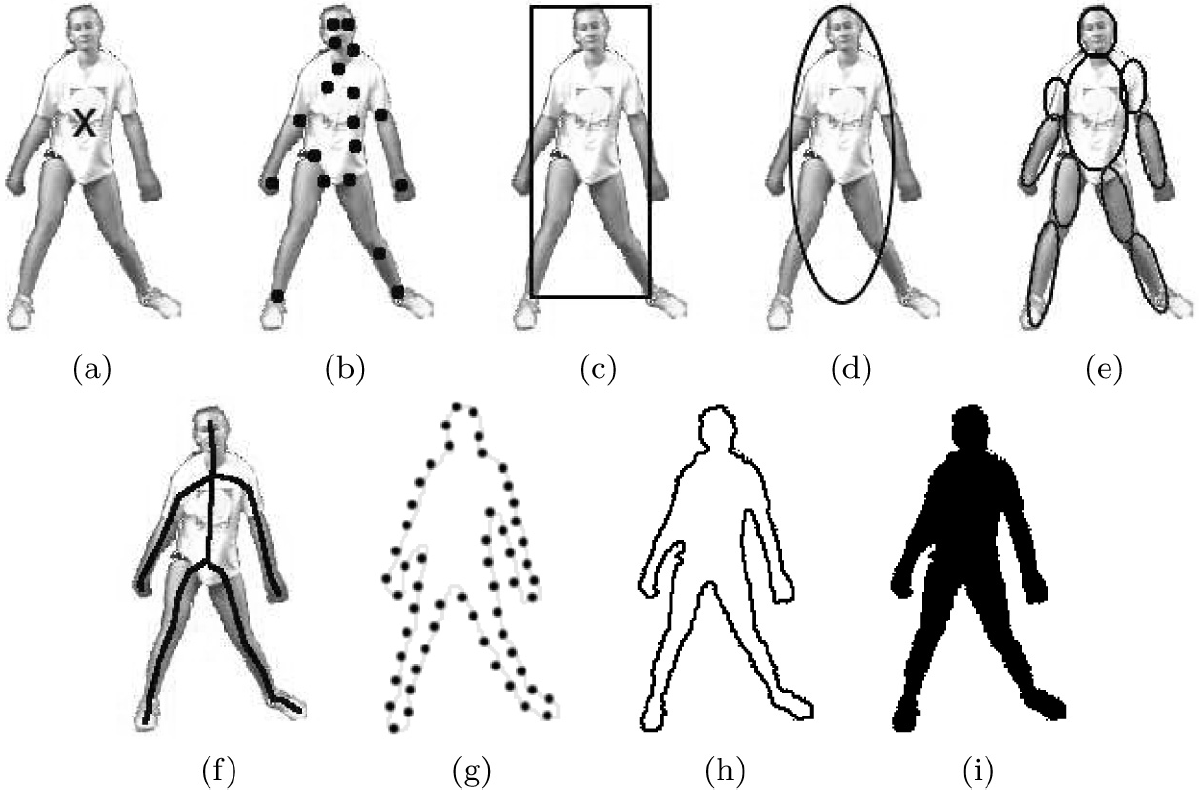
\includegraphics[width=1.0\textwidth]{thesis/2006_JNL_TRKsurvey_Shah_fig1.png}
\caption{Target representations.  (a) Centroid, (b) multiple points,(c) rectangular bounding box, (d) elliptical bounding region, (e) articulated shape model, (f) skeleton, (g) contour control points, (h) contour, (i) silhouette \cite{2006_JNL_SURVEYtrk_Yilmaz}.}
\label{fig:TRK_objectRepresentations}
\end{figure}
\end{frame}


%---------------------------------------------------------
\subsection{(c) Computer vision}
%---------------------------------------------------------
\begin{frame}
\frametitle{Pre-processing}
\logoCSIPCPL\mypagenum
	{\color{red}Steps}
	\begin{enumerate}
		\item Downsampling
		\item Normalization
		\item Stabilization
		\item Background modeling
		\item Feature Extraction
	\end{enumerate}
	\vspace{0.3in}
	{\color{red}Features}
	\begin{enumerate}
		\item Color
		\item Edges
		\item Corners
		\item Motion
		\item Texture
		\item Depth
		\item Density
	\end{enumerate}
\end{frame}









\begin{frame}
\frametitle{Region tracking}
\framesubtitle{overview}
\logoCSIPCPL\mypagenum
	\begin{enumerate}
		\item Template matching
			\begin{itemize}
				\item fixed templates: reliable over short durations 
			\end{itemize}
		\item Subspace methods
			\begin{itemize}
				\item usually learned with PCA
				\item model variations in lighting and pose
				\item disadvantages: object specific, training
			\end{itemize}			
		\item Probability density
			\begin{itemize}
				\item robustness under image distortions and occlusions
				\item fast to learn
				\item disadvantage: lack of expressiveness, registration can be difficult
			\end{itemize}
		\item Motion
			\begin{itemize}
				\item optical flow works well for small displacements
				\item block matching for large motion
				\item computing motion vectors is computationally complex
			\end{itemize}
	\end{enumerate}
\end{frame}


%####################################################################################################
\section{III. RVQ}
%####################################################################################################
%--------------------------------------
\subsection{(a) Introduction}
%--------------------------------------

\begin{frame}
\frametitle{Quantization}
\framesubtitle{overview}
\logoCSIPCPL\mypagenum
	\begin{figure}				
		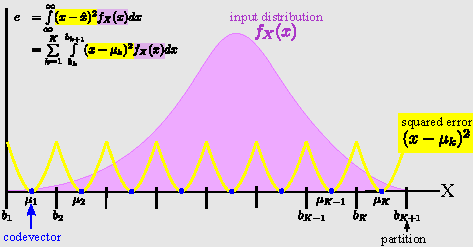
\includegraphics[width=0.9\textwidth]{thesis/Quantization_MSE.pdf}
	\end{figure}
\end{frame}





\begin{frame}[plain]
\frametitle{Lloyd Max conditions}
\framesubtitle{Optimal code-vectors}
\logoCSIPCPL\mypagenum
	\begin{changemargin}{-1.3in}{0in}
		\begin{figure}				
			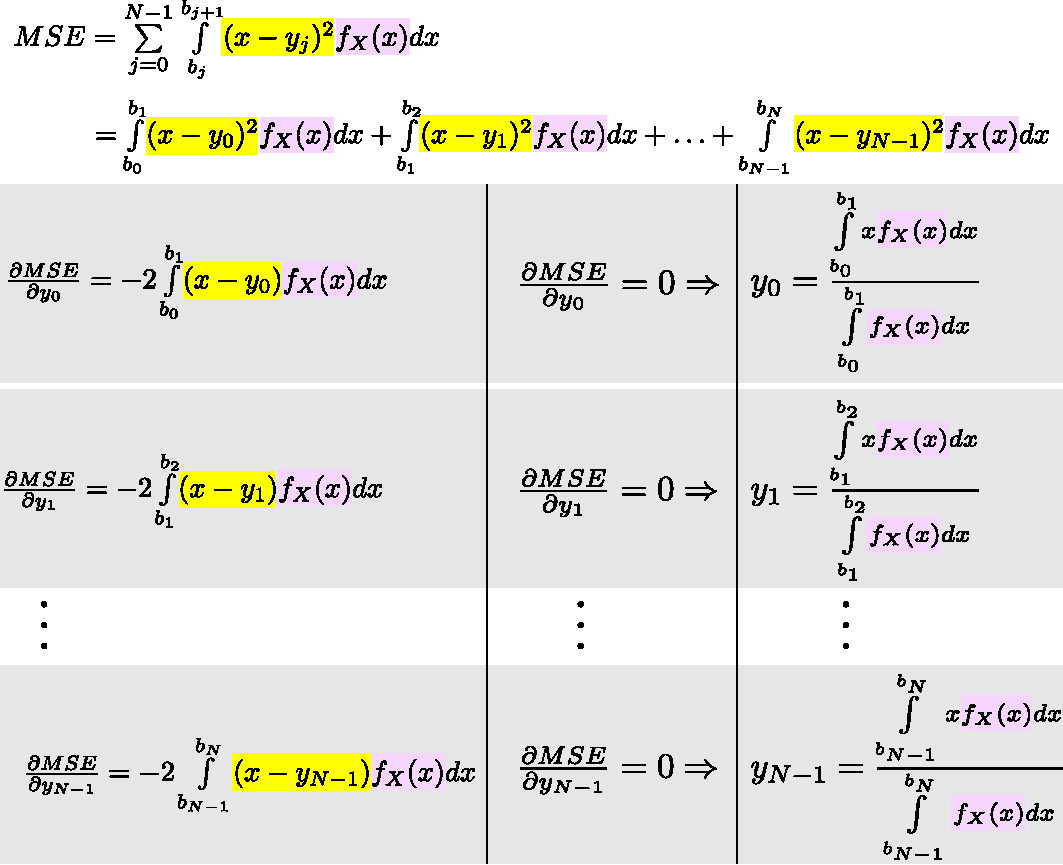
\includegraphics[height=0.8\textheight]{thesis/Quantization_optimalCodevectors.pdf}
		\end{figure}
	\end{changemargin}
\end{frame}



%\begin{frame}
%\frametitle{Lloyd Max conditions}
%\framesubtitle{Optimal partitions}
%\logoCSIPCPL\mypagenum
%	\begin{figure}				
%		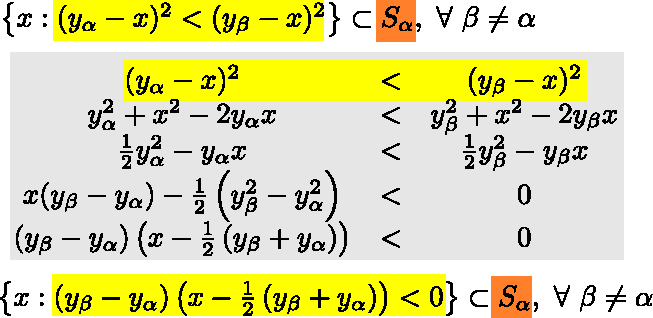
\includegraphics[width=1.0\textwidth]{thesis/Quantization_optimalPartitions.pdf}
%	\end{figure}
%\end{frame}
%
%
%
%\begin{frame}[plain]
%\frametitle{Lloyd Max conditions}
%\framesubtitle{Optimal partitions (cont.)}
%\logoCSIPCPL\mypagenum
%	\begin{changemargin}{-1.3in}{0in}
%		\begin{figure}				
%			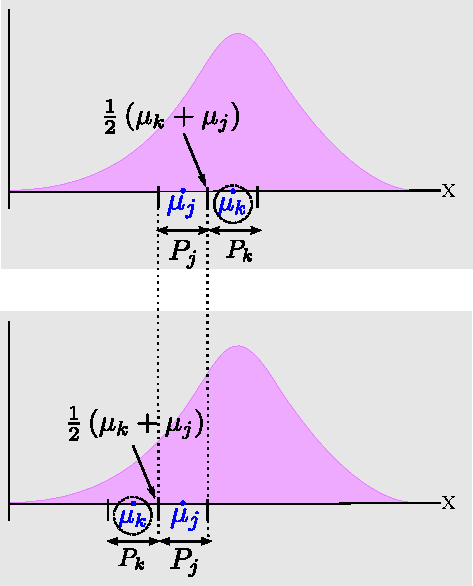
\includegraphics[height=0.8\textheight]{thesis/Quantization_optimalPartitions2.pdf}
%		\end{figure}
%	\end{changemargin}
%\end{frame}


\begin{frame}
\frametitle{Vector Quantization}
\framesubtitle{types}
\logoCSIPCPL\mypagenum
	\begin{itemize}
		\item Unstructured
			\begin{itemize}
				\item Exhaustive Search (ESVQ)
			\end{itemize}
		\item Structured
		\begin{itemize}
			\item Tree Structured (TSVQ)
			\item Transform
			\item Product
				\begin{itemize}
					\item Mean-removed
					\item Shape-gain
					\item Residual (RVQ)
				\end{itemize}
		\end{itemize}
	\end{itemize}
\end{frame}




\begin{frame}[plain]
\frametitle{RVQ}
\framesubtitle{block diagram}
\logoCSIPCPL\mypagenum
	\begin{changemargin}{-1.3in}{0in}
		\begin{figure}				
			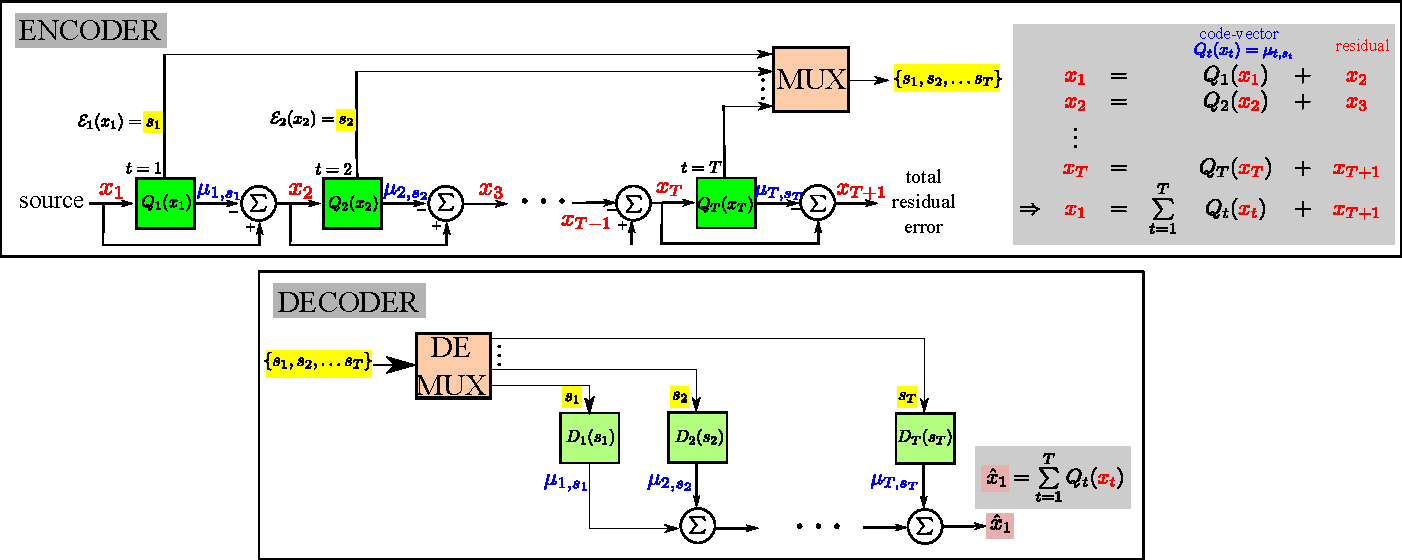
\includegraphics[width=1.3\textwidth]{thesis/RVQ_blockDiagram.pdf}
		\end{figure}
	\end{changemargin}
\end{frame}


%\begin{frame}
%\frametitle{RVQ}
%\framesubtitle{distortion}
%\logoCSIPCPL\mypagenum
%	\begin{figure}				
%		\includegraphics[width=1.0\textwidth]{thesis/RVQ_distortion.pdf}
%	\end{figure}
%\end{frame}



\begin{frame}
\frametitle{RVQ}
\framesubtitle{tree structure}
\logoCSIPCPL\mypagenum
	\begin{figure}				
		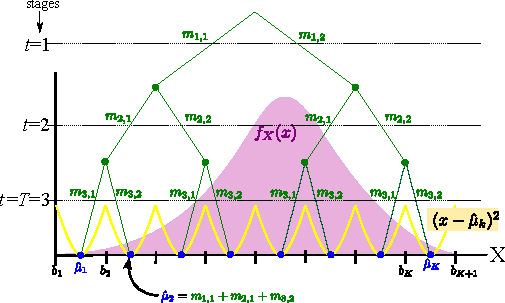
\includegraphics[width=1.0\textwidth]{thesis/RVQ_graphicalReconstruction.pdf}
	\end{figure}
\end{frame}




\begin{frame}[plain]
\frametitle{RVQ}
\framesubtitle{derivation}
\logoCSIPCPL\mypagenum
	\begin{changemargin}{-1.3in}{0in}
		\begin{figure}				
			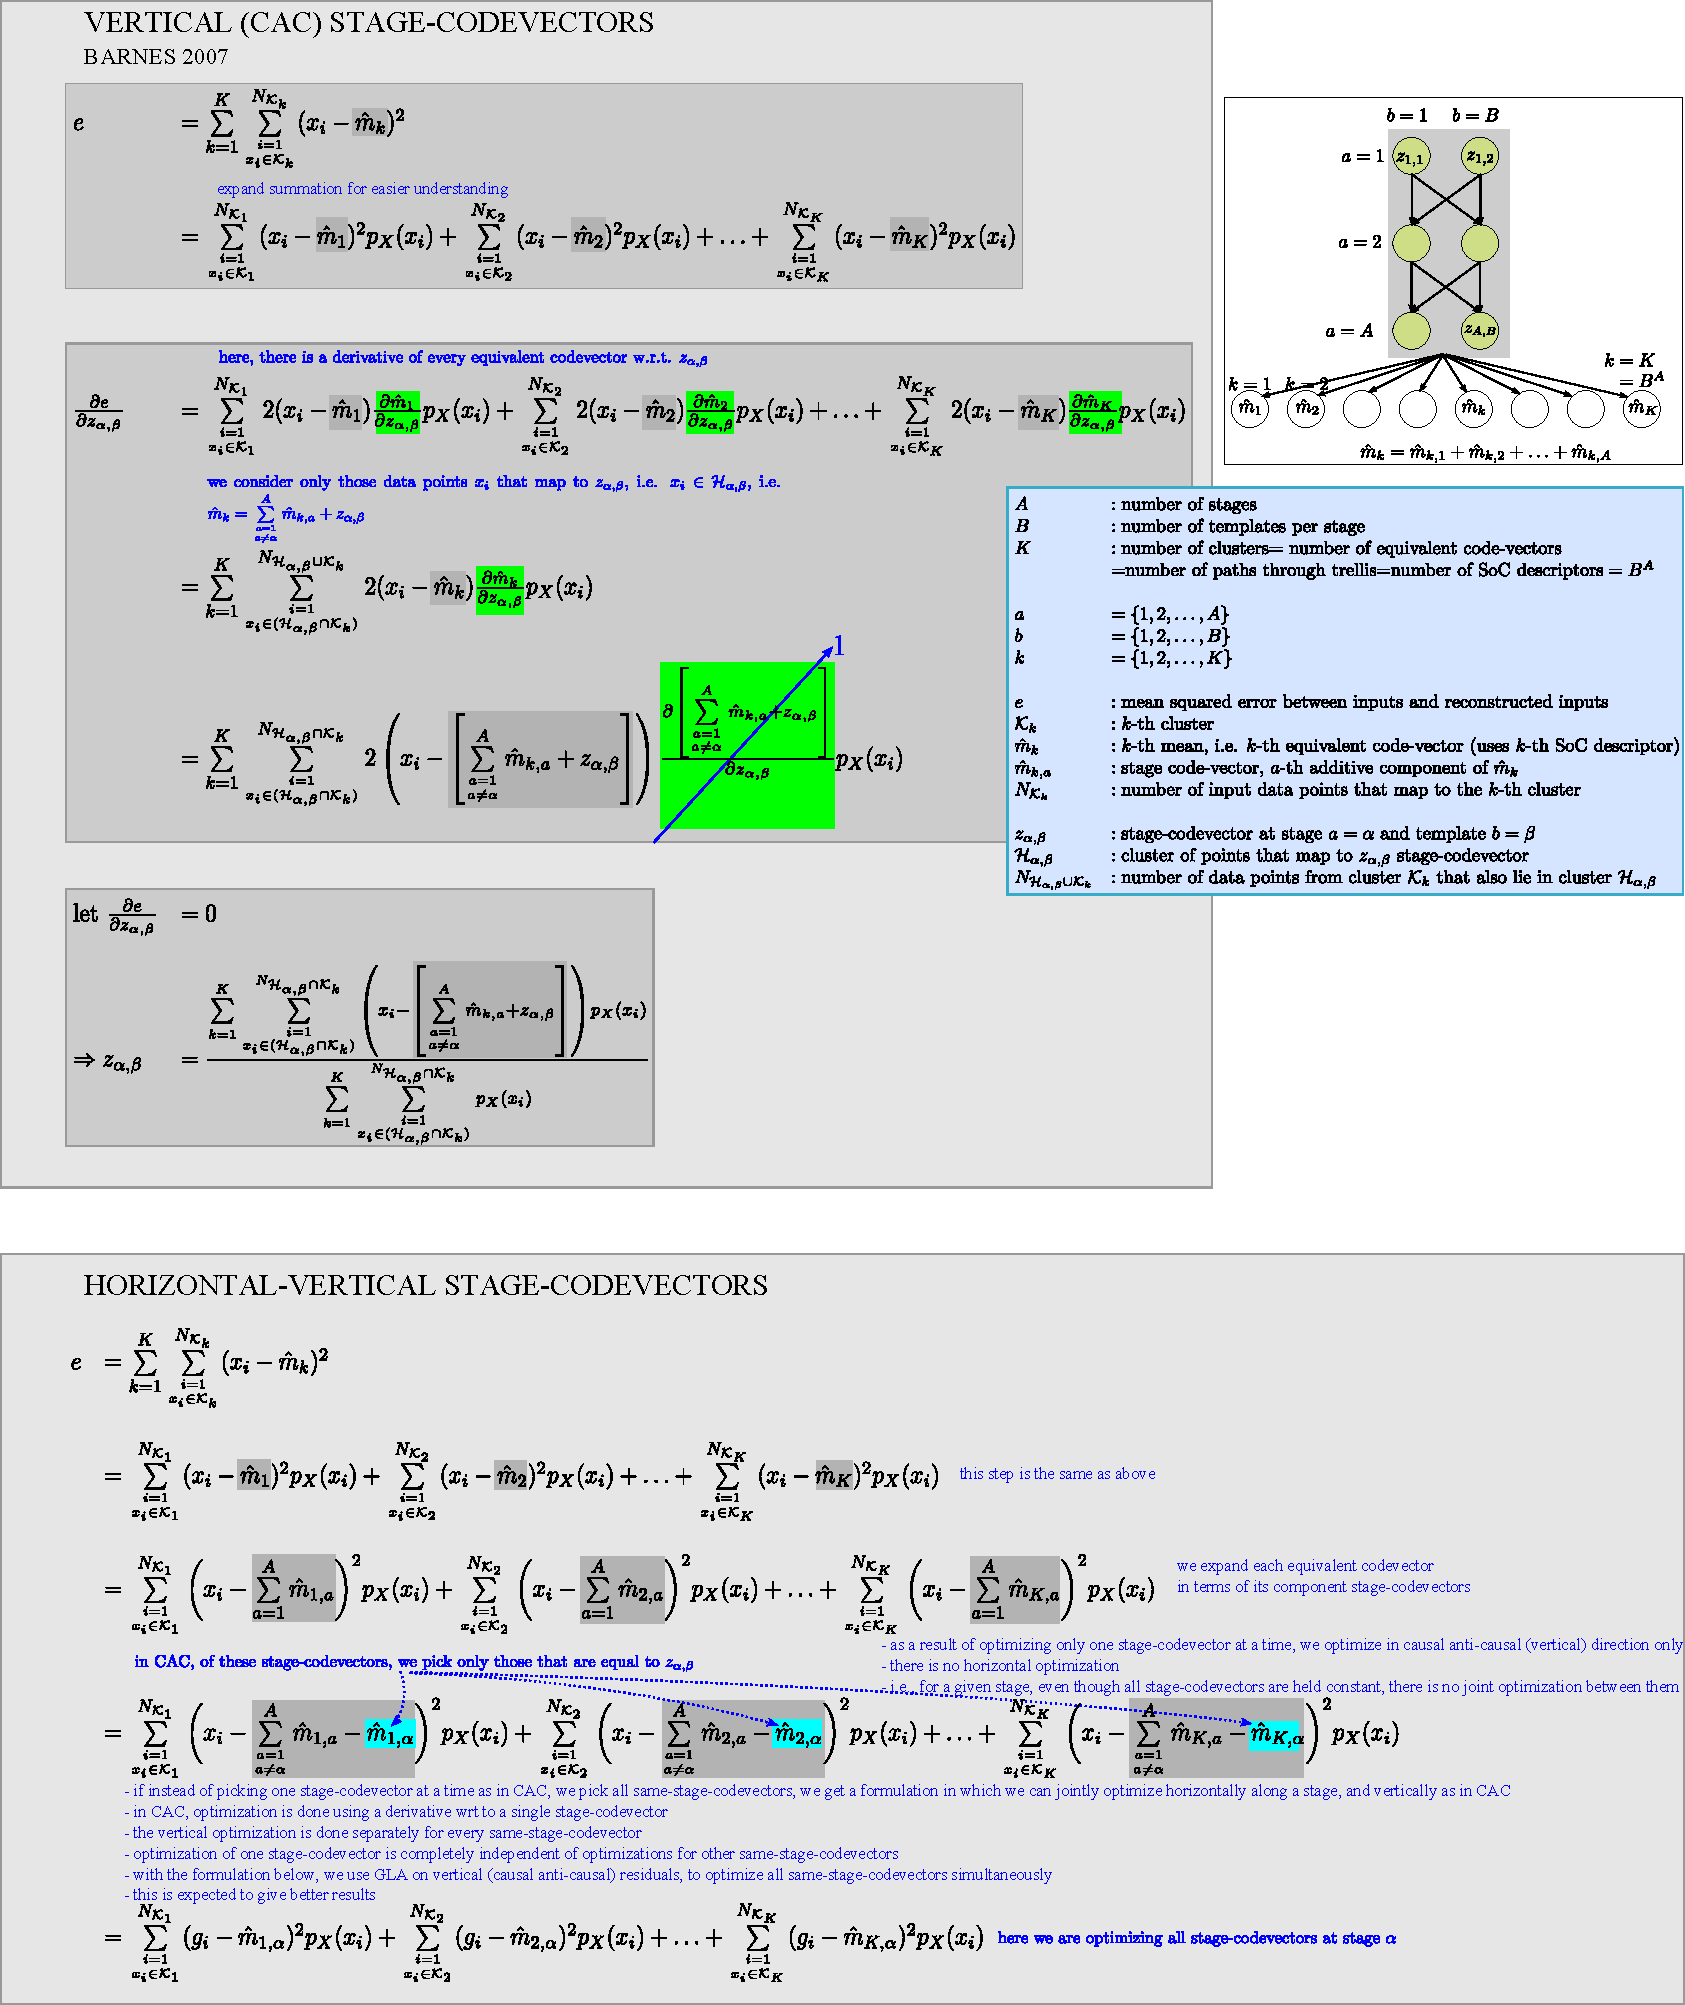
\includegraphics[width=1.3\textwidth]{thesis/RVQ_CAC_derivation.pdf}
		\end{figure}
	\end{changemargin}
\end{frame}


%--------------------------------------
\subsection{(b) Comparisons}
%--------------------------------------
\begin{frame}
\frametitle{RVQ comparison}\logoCSIPCPL\mypagenum
\framesubtitle{1. with ESVQ}
	\begin{itemize}
		\item ESVQ
			\begin{itemize}
				\item $N=2^{rk}$ code-vectors
				\item Computations: $O(2^{rk})$
				\item Memory: $O(2^{rk})$
				\item Exponential in computations and memory
			\end{itemize}
		\item RVQ
			\begin{itemize}
				\item $N={M^P}$ code-vectors
				\item M code-vectors for each of P stages
				\item Computations: $O(MP)$
				\item Memory: $O(MP)$
				\item Linear in computations and memory
			\end{itemize}
	\end{itemize}
	Generally, structurally constrained quantizers cannot provide performance as good as ESVQ
	\begin{itemize}
		\item RVQ can handle higher dimensions due to linear complexity
		\item Better performance than ESVQ possible, for given implementation cost
	\end{itemize}	
\end{frame}


\begin{frame}[plain]
\frametitle{RVQ comparison}
\framesubtitle{2. with TSVQ}
\logoCSIPCPL\mypagenum
%	\begin{changemargin}{-1.3in}{0in}
%		\begin{figure}				
%			\includegraphics[width=1.3\textwidth]{thesis/RVQ_comparisonWithTSVQ.pdf}
%		\end{figure}
%	\end{changemargin}
\end{frame}



%\begin{frame}[plain]
%\frametitle{RVQ comparison}
%\framesubtitle{3. with PCA}
%\logoCSIPCPL\mypagenum
%	\begin{changemargin}{-1.3in}{0in}
%		\begin{figure}				
%			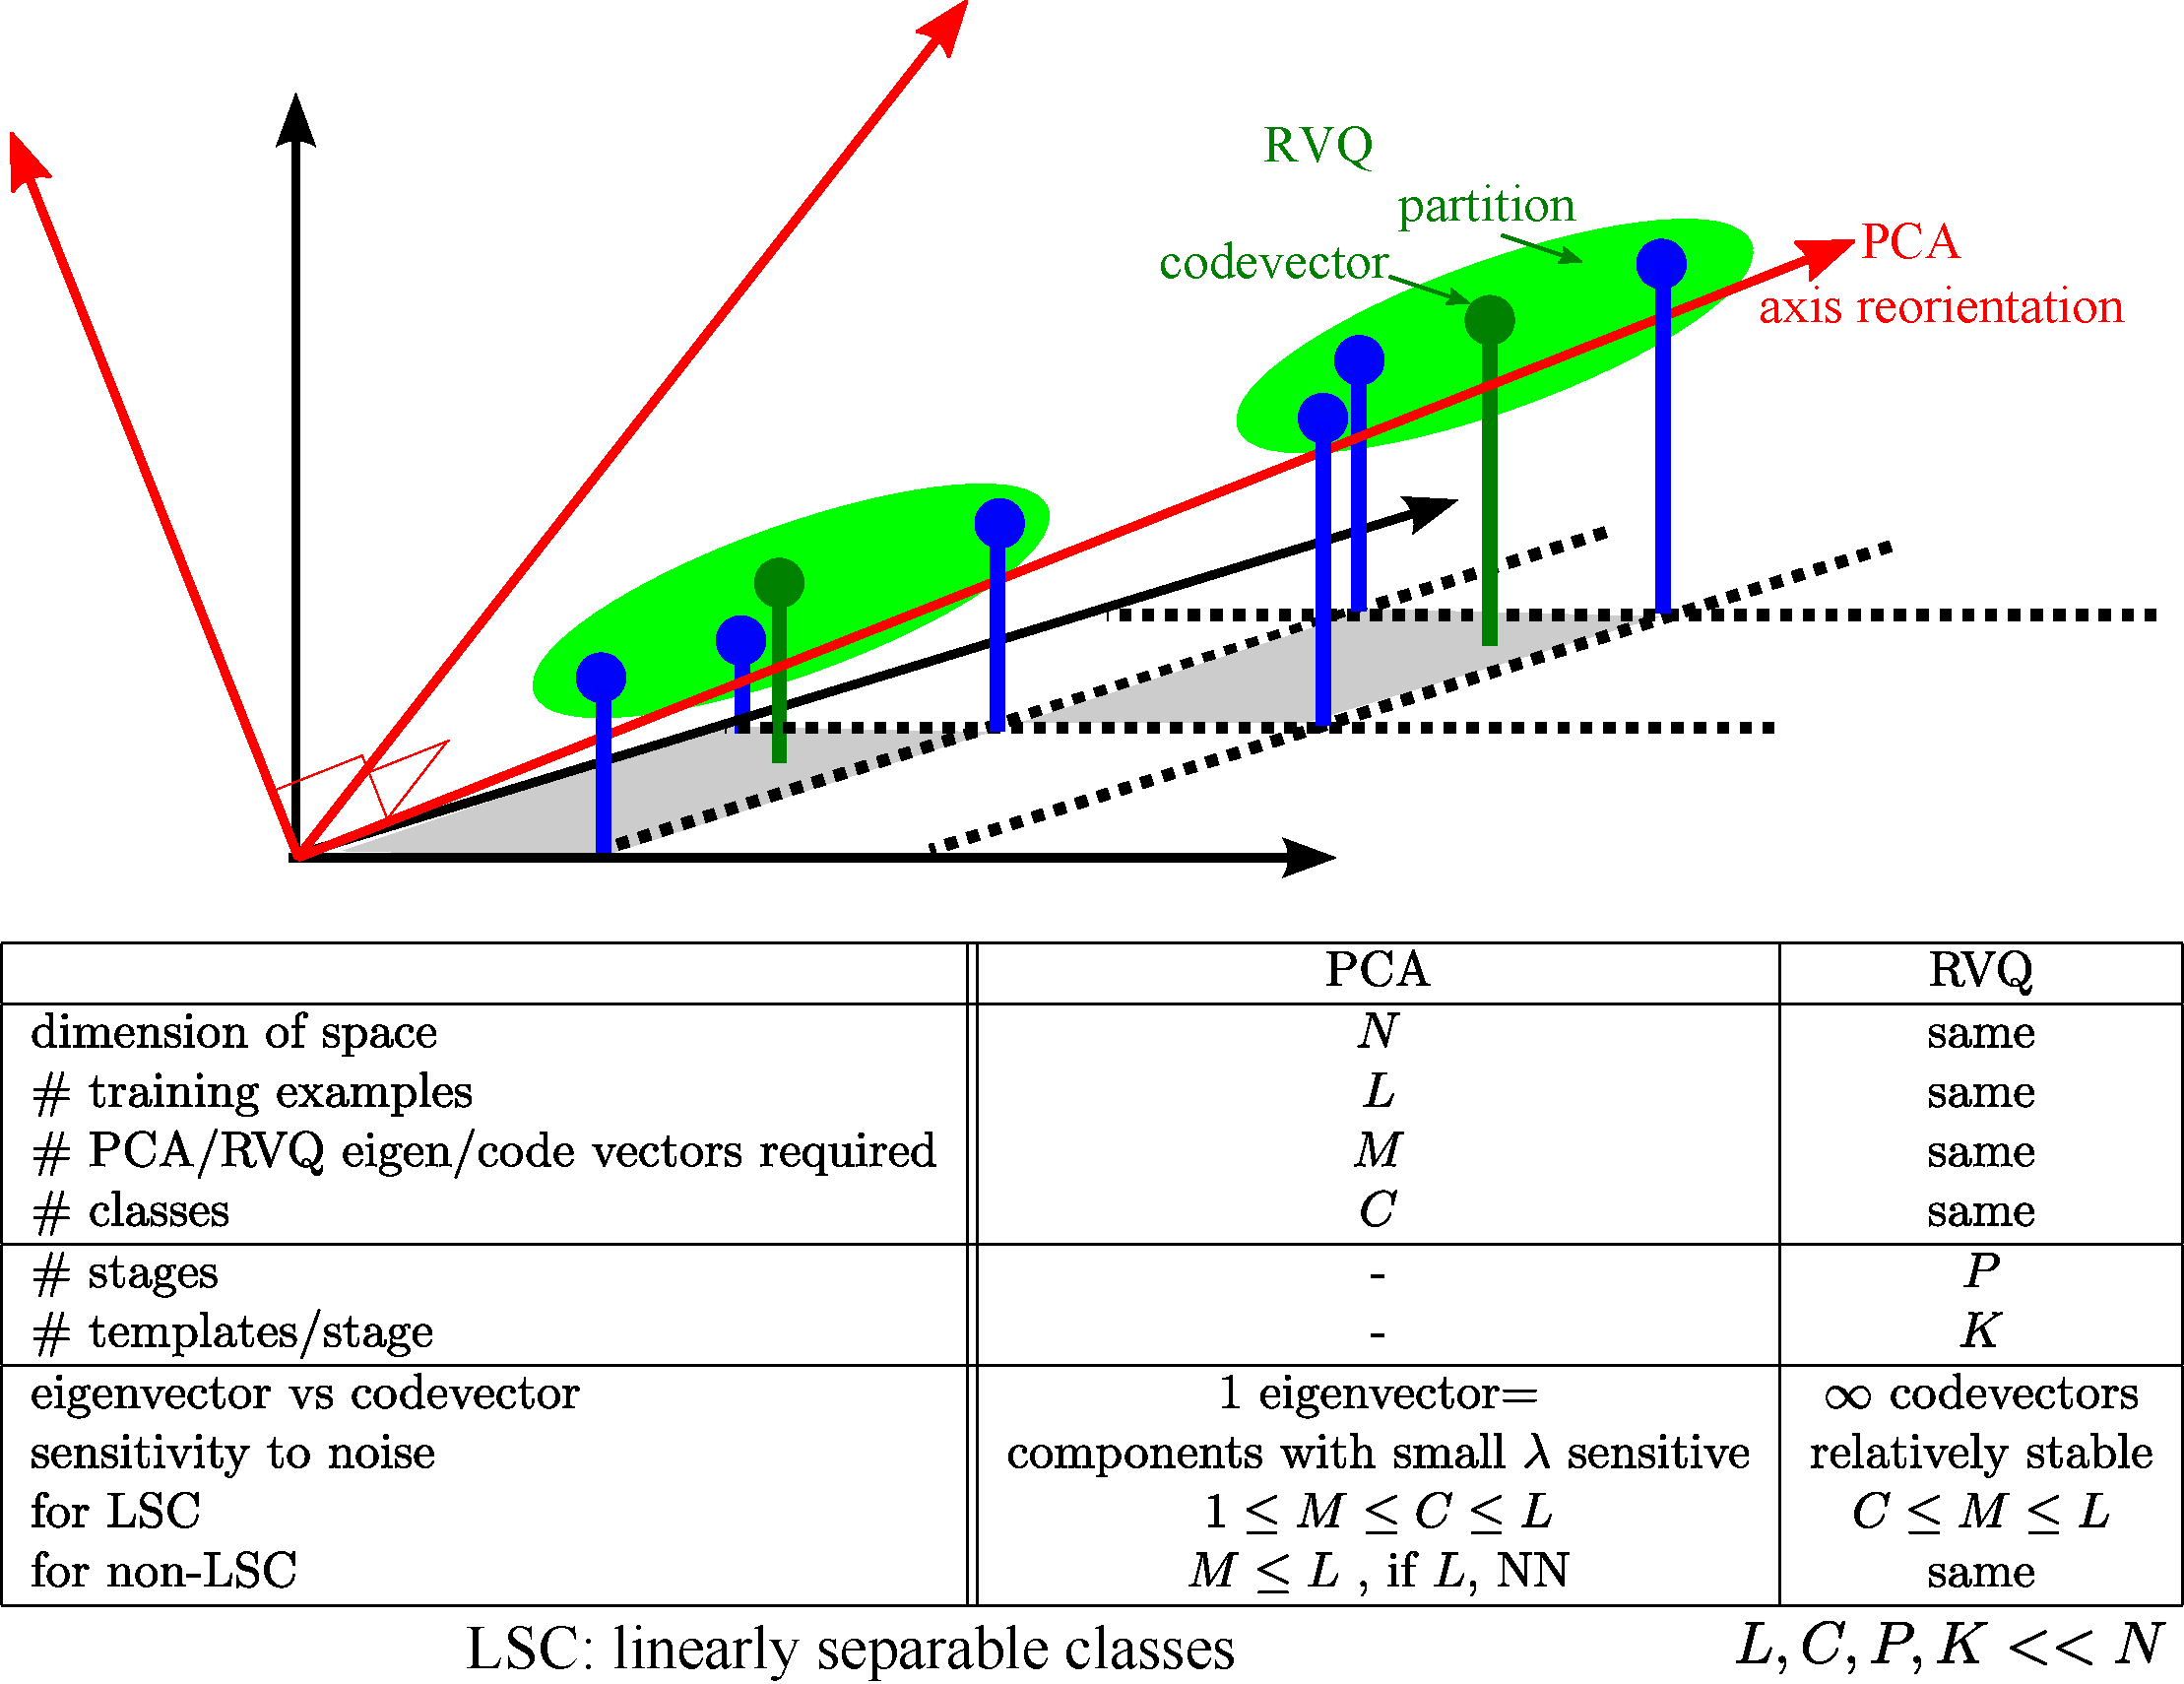
\includegraphics[width=1.3\textwidth]{thesis/RVQ_comparisonWithPCA.pdf}
%		\end{figure}
%	\end{changemargin}
%\end{frame}


%--------------------------------------------------------
\subsection{(c) Image classification}
%--------------------------------------------------------




\begin{frame}
\frametitle{RVQ classification}
\framesubtitle{\small Satellite imagery: pre-Tsunami Sri Lanka \\(training phase)}
\logoCSIPCPL\mypagenum
	\begin{figure}		
		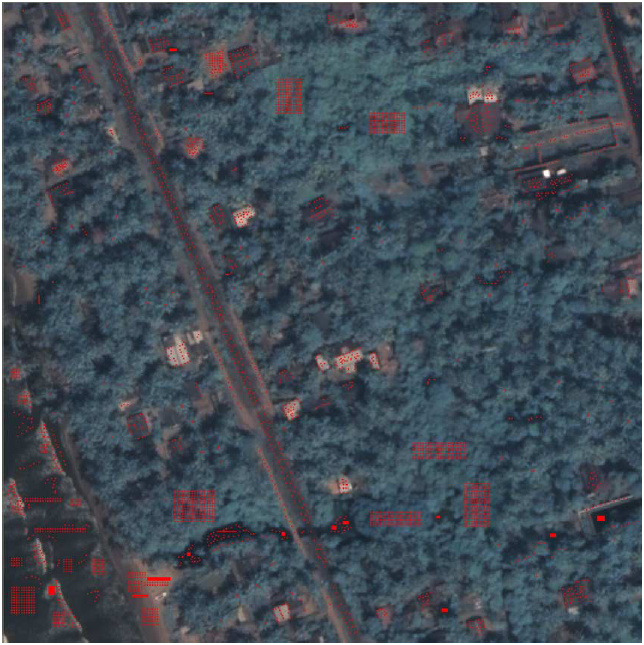
\includegraphics[height=0.35\textheight]{thesis/RVQ_SatelliteSriLanka_1_snippets.png}			
	\end{figure}
	\begin{figure}		
		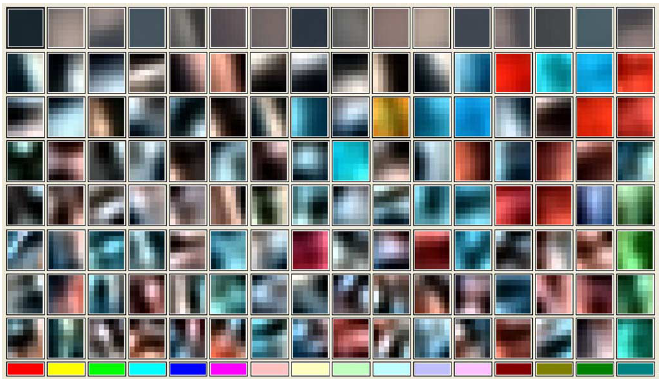
\includegraphics[height=0.40\textheight]{thesis/RVQ_SatelliteSriLanka_2_codebooks.png}			
	\end{figure}
\end{frame}




\begin{frame}
\frametitle{RVQ classification}
\framesubtitle{\small Satellite imagery: pre-Tsunami Sri Lanka\\(testing phase)}
\logoCSIPCPL\mypagenum
	\begin{figure}		
		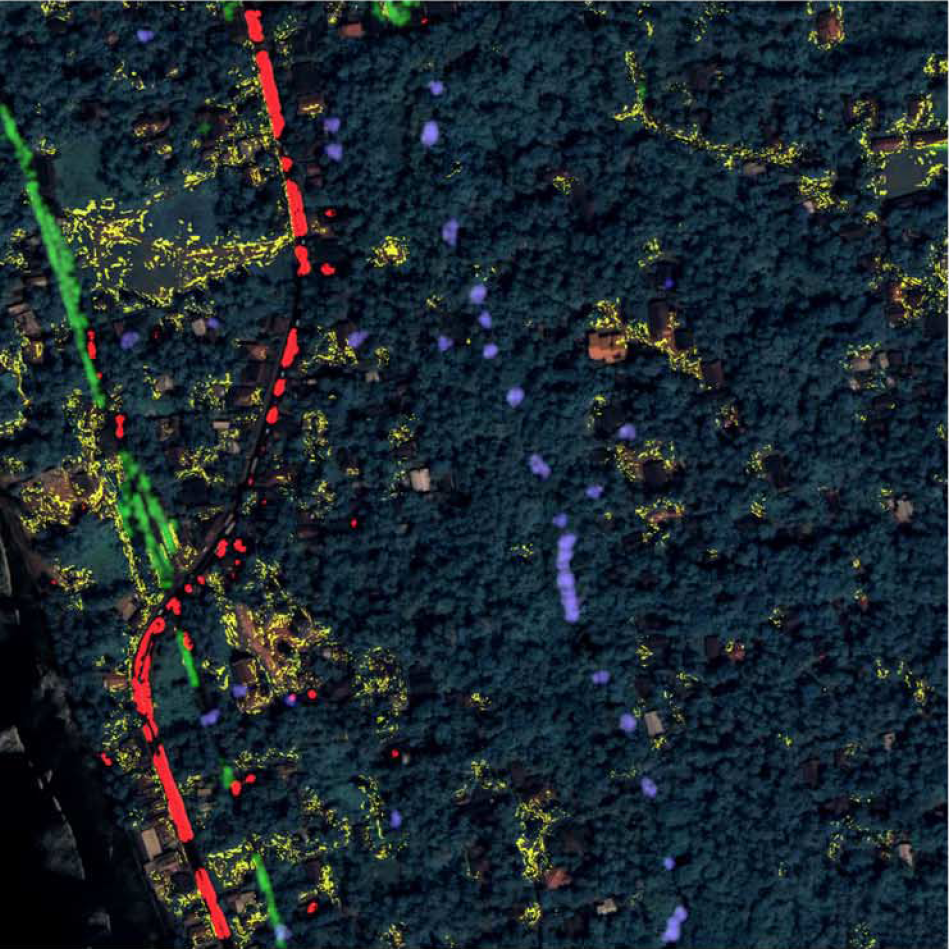
\includegraphics[height=0.6\textheight]{thesis/RVQ_SatelliteSriLanka_3_labeling.png}
		\caption{\hspace{1.3in}{\color{yellow}yellow}: dirt paths \\\hspace{1.3in}{\color{blue}blue}: rivers \\\hspace{1.3in}{\color{red}red}: paved roads \\\hspace{1.3in}{\color{green}green}: train tracks}
	\end{figure}
\end{frame}


%=======================================
\section{IV. RVQ tracking}
%=======================================
\begin{frame}
\frametitle{Experimental overview}
\framesubtitle{}
\logoCSIPCPL\mypagenum
\setcounter{subfigure}{0}
\begin{figure}[t]
\centering
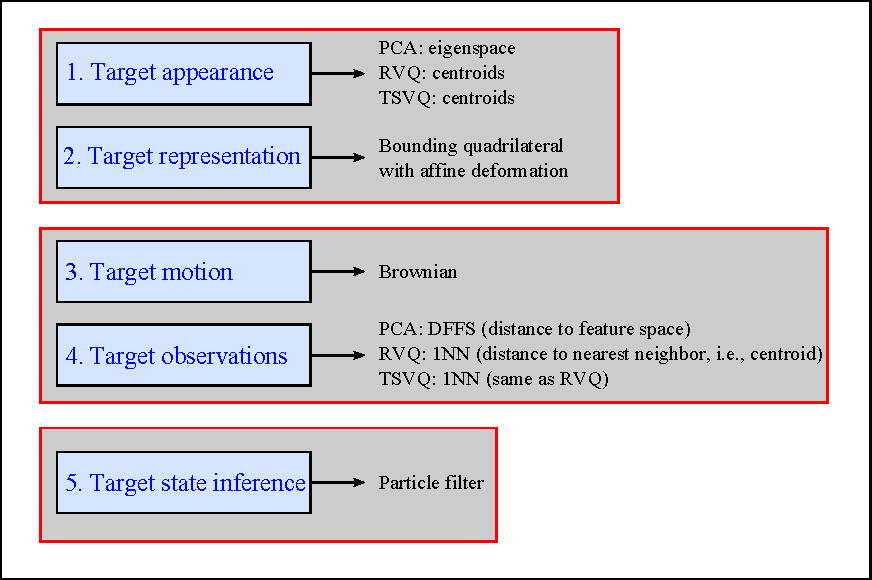
\includegraphics[width=1.0\textwidth]{thesis/PhD_experimentalOverview.pdf}
\label{fig:overview}
\end{figure}
\end{frame}



\begin{frame}[plain]
\frametitle{Temporal evolution}
\framesubtitle{}
\logoCSIPCPL\mypagenum
\setcounter{subfigure}{0}
\begin{changemargin}{-1.3in}{0in}
\begin{figure}[t]
\centering
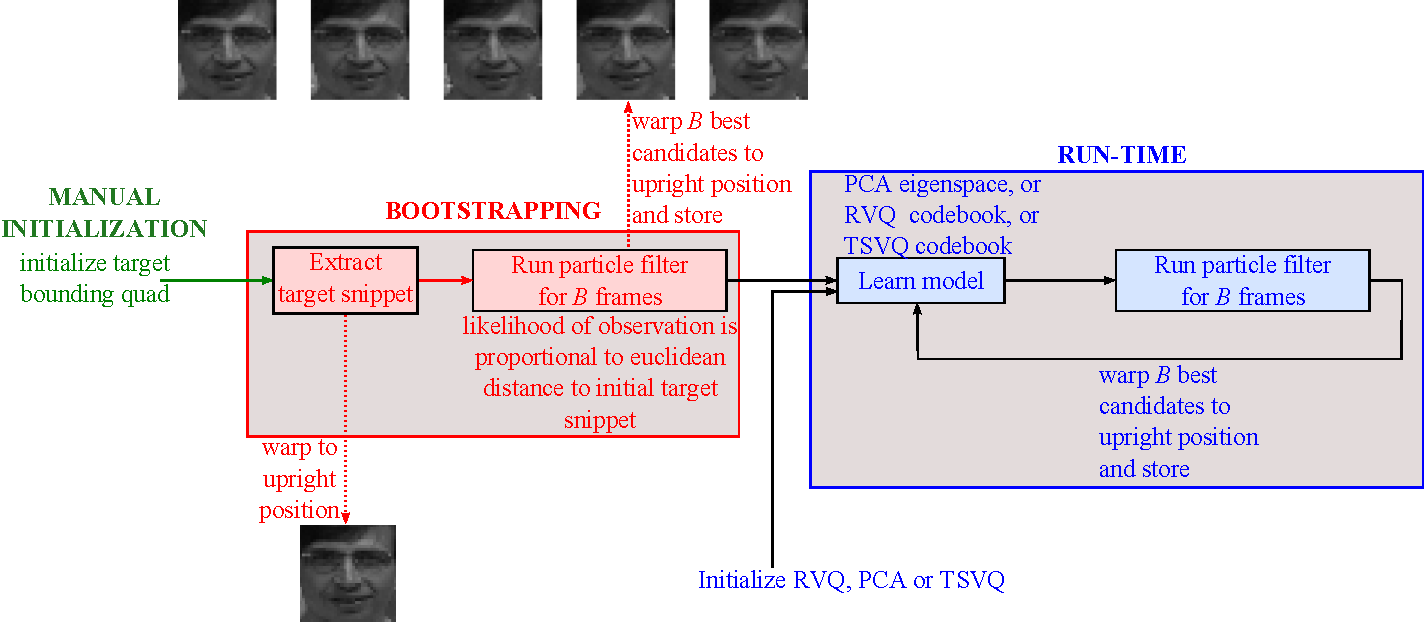
\includegraphics[width=1.3\textwidth]{thesis/PhD_experimentalTemporalOverview.pdf}
\label{fig:temporal_overview}
\end{figure}
\end{changemargin}
\end{frame}


\begin{frame}
\frametitle{Publicly available datasets\footnote{Ross et. al. 2008}}
\framesubtitle{Dudek, davidin300, sylv, fish, car4, car11}
\logoCSIPCPL\mypagenum
\setcounter{subfigure}{0}
\begin{figure}[h!]
\centering\subfigure{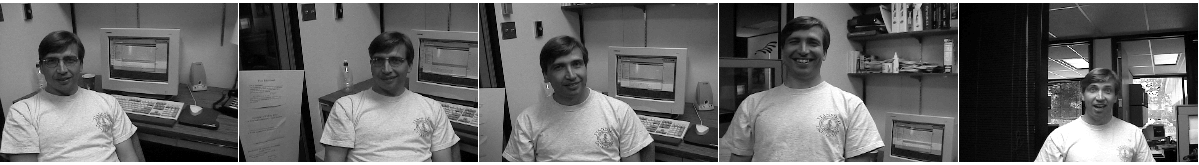
\includegraphics[height=0.41in]{thesis/seq_1_Dudek.png}\label{fig:trk_pca_1a}}
\subfigure{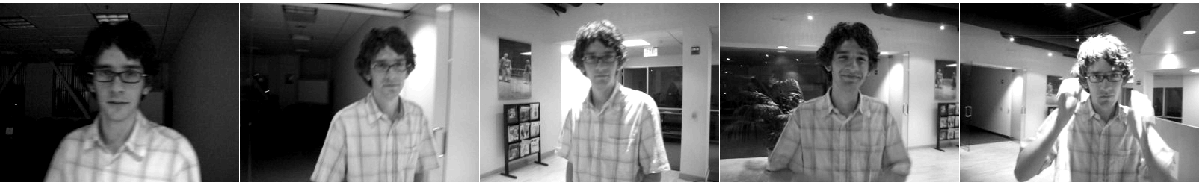
\includegraphics[height=0.41in]{thesis/seq_2_davidin300.png}\label{fig:trk_pca_1b}}
\subfigure{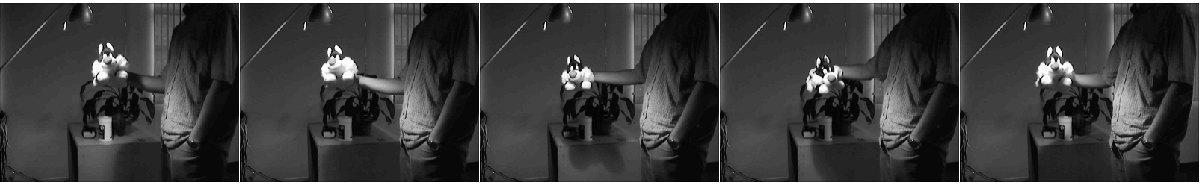
\includegraphics[height=0.41in]{thesis/seq_3_sylv.png}\label{fig:trk_pca_1c}}
\subfigure{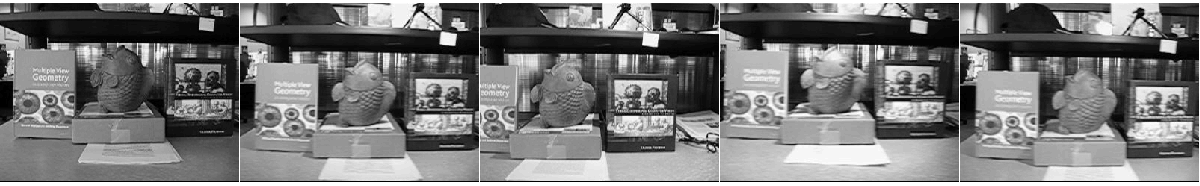
\includegraphics[height=0.41in]{thesis/seq_5_fish.png}\label{fig:trk_pca_1d}}
\subfigure{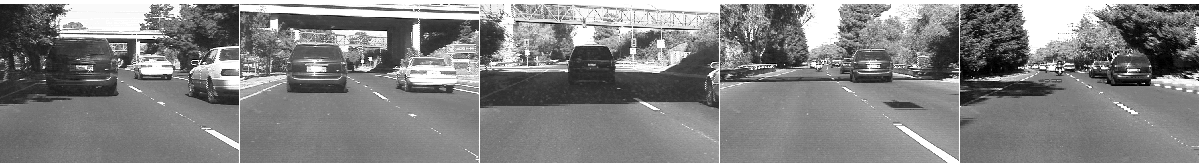
\includegraphics[height=0.41in]{thesis/seq_6_car4.png}\label{fig:trk_pca_1d}}
\subfigure{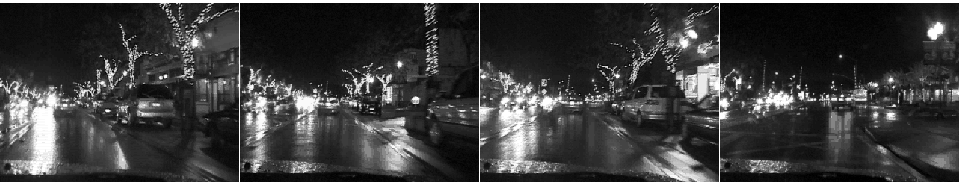
\includegraphics[height=0.41in]{thesis/seq_7_car11.png}\label{fig:trk_pca_1d}}
\label{fig:trk_sequences}
\end{figure}
\end{frame}


%------------------------------------------------------
\subsection{(a) Appearance model}
%------------------------------------------------------

%PCA
\begin{frame}
\frametitle{PCA}
\framesubtitle{80/20 cross-validation, 10 runs, $\mathbb{R}^{1089}$}
\logoCSIPCPL\mypagenum
\setcounter{subfigure}{0}
\begin{figure}[t]
\subfigure[Uniform.]{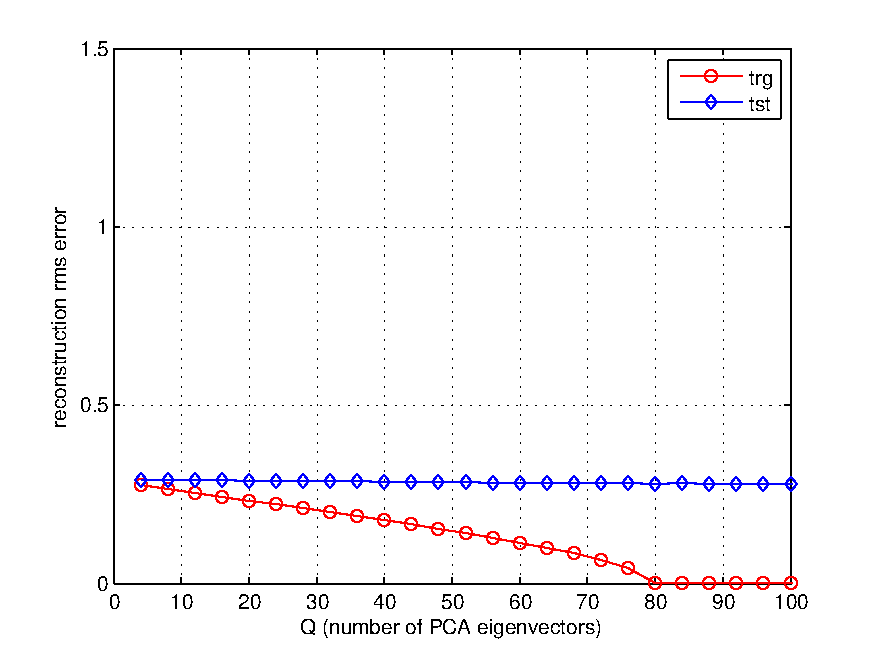
\includegraphics[width=0.45\textwidth]{thesis/PCA_Uniform.pdf}}
\subfigure[Gaussian.]{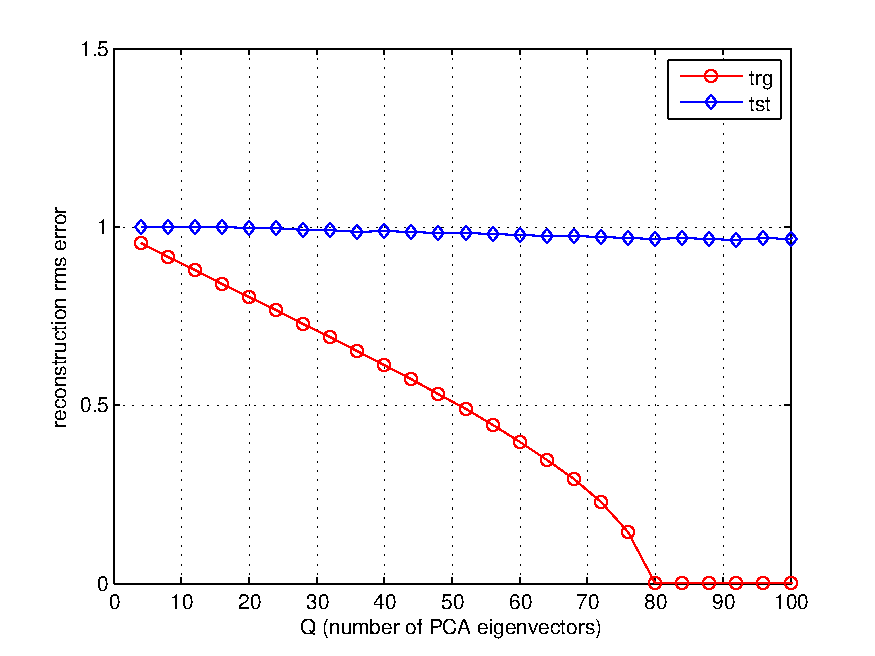
\includegraphics[width=0.45\textwidth]{thesis/PCA_Gaussian.pdf}}
\subfigure[Gauss-Markov.]{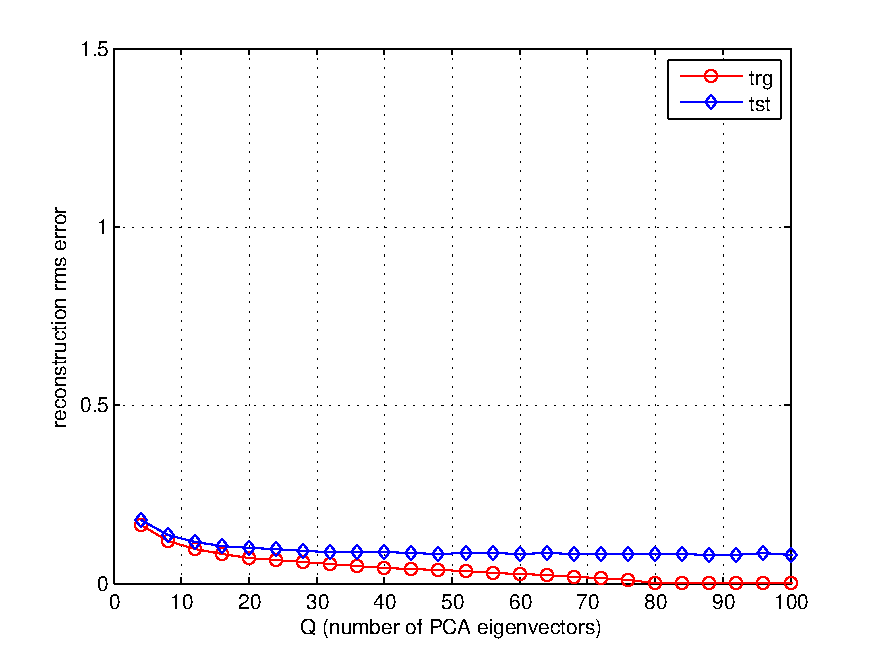
\includegraphics[width=0.45\textwidth]{thesis/PCA_GaussMarkov.pdf}}
\subfigure[Dudek sequence.]{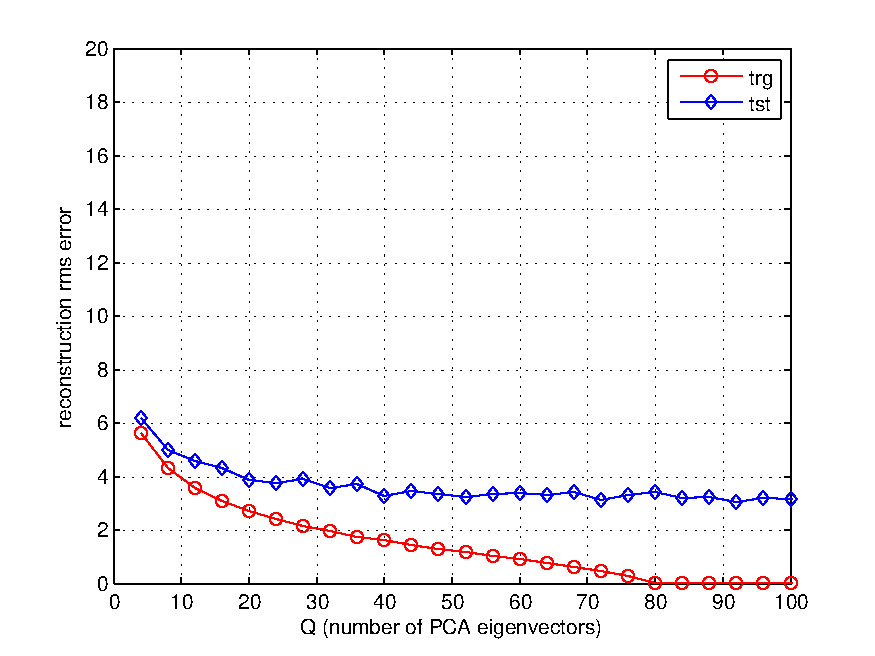
\includegraphics[width=0.45\textwidth]{thesis/PCA_Dudek.pdf}}
\label{fig:PCA_results}
\end{figure}
\end{frame}

%RVQ appearance model (varying P)
\begin{frame}
\frametitle{RVQ, $M=4$, varying $P$}
\framesubtitle{80/20 cross-validation, 10 runs, $\mathbb{R}^{1089}$}
\logoCSIPCPL\mypagenum
\setcounter{subfigure}{0}
\begin{figure}
\subfigure[Uniform.]
{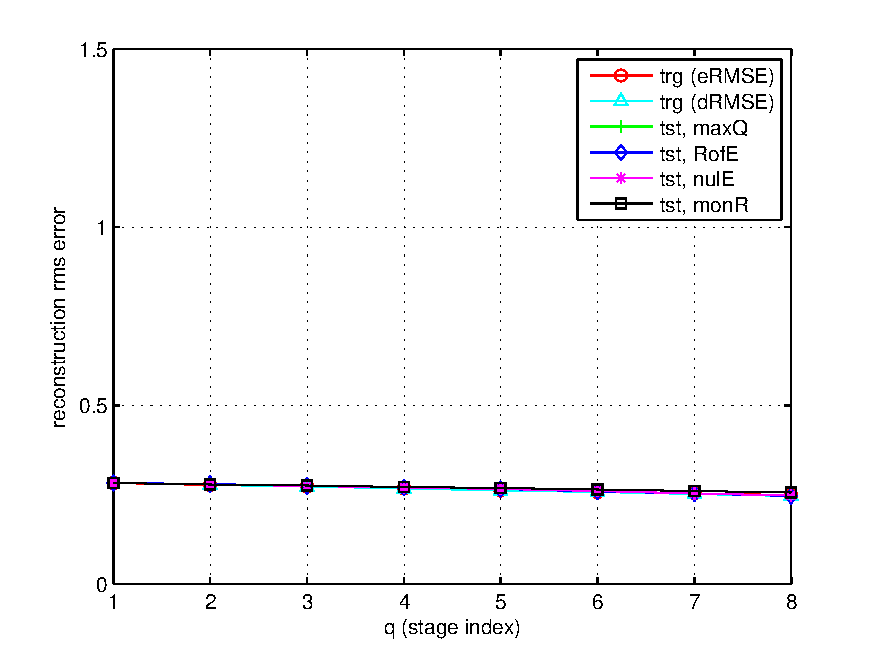
\includegraphics[width=0.45\textwidth]{thesis/RVQ_8x4_Uniform.pdf}}
\subfigure[Gaussian.]
{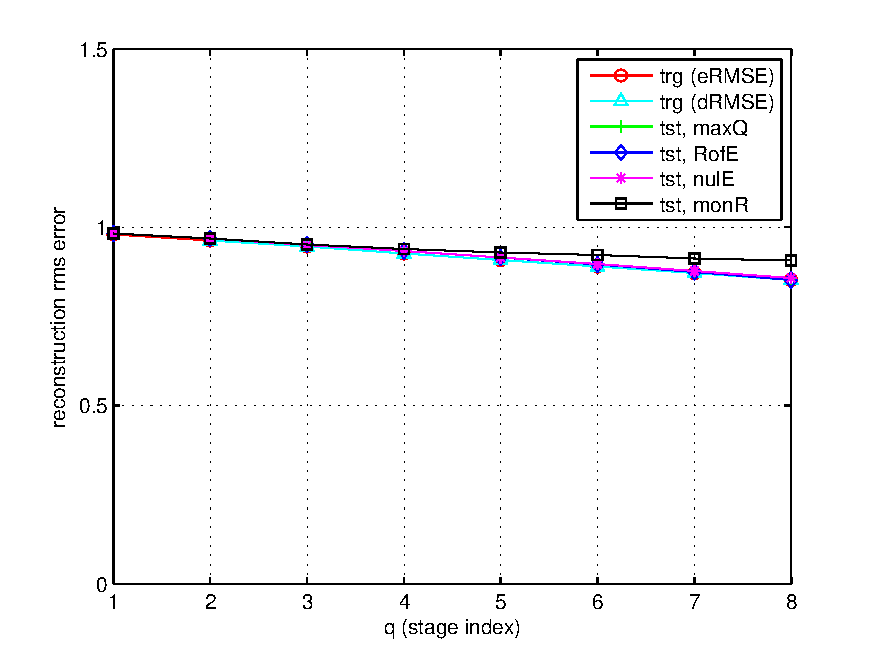
\includegraphics[width=0.45\textwidth]{thesis/RVQ_8x4_Gaussian.pdf}}
\subfigure[Gauss-Markov.]
{\includegraphics[width=0.45\textwidth]{thesis/RVQ_8x4_GaussMarkov.pdf}}
\subfigure[Dudek sequence.]
{\includegraphics[width=0.45\textwidth]{thesis/RVQ_8x4_Dudek.pdf}}
\end{figure}
\end{frame}


%TSVQ
\begin{frame}
\frametitle{TSVQ (binary, balanced-tree)}
\framesubtitle{80/20 cross-validation, 10 runs, $\mathbb{R}^{1089}$}
\logoCSIPCPL\mypagenum
\setcounter{subfigure}{0}
\begin{figure}[t]
\subfigure[Uniform.]{\includegraphics[width=0.45\textwidth]{thesis/TSVQ_Uniform.pdf}}
\subfigure[Gaussian.]{\includegraphics[width=0.45\textwidth]{thesis/TSVQ_Gaussian.pdf}}
\subfigure[Gauss-Markov.]{\includegraphics[width=0.45\textwidth]{thesis/TSVQ_GaussMarkov.pdf}}
\subfigure[Dudek sequence.]{\includegraphics[width=0.45\textwidth]{thesis/TSVQ_Dudek.pdf}}
\label{fig:TSVQ_results}
\end{figure}
\end{frame}




%RVQ appearance model (varying M)
\begin{frame} 
\frametitle{RVQ, $P=8$, varying $M$}
\framesubtitle{80/20 cross-validation, 10 runs, $\mathbb{R}^{1089}$}
\logoCSIPCPL\mypagenum
\setcounter{subfigure}{0}
\begin{figure}[t]
\subfigure[Uniform.]
{\includegraphics[width=0.45\textwidth]{thesis/RVQ_uniform.pdf}}
\subfigure[Gaussian.]
{\includegraphics[width=0.45\textwidth]{thesis/RVQ_Gaussian.pdf}}
\subfigure[Gauss-Markov.]
{\includegraphics[width=0.45\textwidth]{thesis/RVQ_GaussMarkov.pdf}}
\subfigure[Dudek sequence.]
{\includegraphics[width=0.45\textwidth]{thesis/RVQ_Dudek.pdf}}
\label{fig:RVQ_results_varyingM}
\end{figure}
\end{frame}


%------------------------------------------------------
\subsection{(b) Observation model}
%------------------------------------------------------


%------------------------------------------------------
\subsection{(c) Representation model}
%------------------------------------------------------
\begin{frame}[plain]
\frametitle{RVQ, $P=8$, varying $M$}
\framesubtitle{80/20 cross-validation, 10 runs, $\mathbb{R}^{1089}$}
\logoCSIPCPL\mypagenum
\scriptsize
\begin{changemargin}{-1.3in}{0in}
\begin{equation}
\begin{array}{llllllll}
\mathbf{A} &= \left[\begin{array}{lll}a & b \\ c & d\\ \end{array}\right] \\
&=\mathbf{U}{\color{darkgreen}\mathbf{S}}{\color{red}\mathbf{V}^t} \\
&={\color{blue}(\mathbf{U}\mathbf{V}^t)}{\color{red}\mathbf{V}}{\color{darkgreen}\mathbf{S}}{\color{red}\mathbf{V}^t}\\
&={\color{blue}\mathbf{R}(\theta)}{\color{red}\mathbf{R}(-\phi)}{\color{darkgreen}\mathbf{S}}{\color{red}\mathbf{R} (\phi)}\\
&={\color{blue}\RotMatrixTheta}{\color{red}\RotMatrixminusPhi}{\color{darkgreen}\EigenvalueMatrix}{\color{red}\RotMatrixPhi}\\\\
\end{array}
\label{Eq:AffineDecomposition}
\end{equation}
\end{changemargin}
\end{frame}



\begin{frame}
\frametitle{Inverse affine transform}
\framesubtitle{one time initialization}
\logoCSIPCPL\mypagenum
In first frame
\begin{itemize}
\item given target affine parameters and ground truth feature points
\item apply inverse affine transform on ground truth points to warp them to canonical position, and save this position $(\mathbf{x, y})$
\end{itemize}
\begin{figure}[t]
\centering
\includegraphics[width=0.6\textwidth]{figs/dataset_Dudek_00001_inverseAffine.pdf}
\label{fig:original_feature_points}
\end{figure}
\end{frame}




%------------------------------------------------------
\subsection{(d) Motion model}
%------------------------------------------------------
\begin{frame}
\frametitle{Generating track candidates}
\framesubtitle{use random affine deformation to model motion}
\logoCSIPCPL\mypagenum
During run-time
\begin{itemize}
\item Perturb affine parameters
\item For each affine set, 
\begin{itemize}
\item apply forward affine transform on zero-centered canonical grid 
\item bilinear interpolation to extract ROI, one per affine set, as shown below
\begin{figure}[t]
\centering
\includegraphics[width=0.35\textwidth]{figs/affineCandidates.pdf}
\label{Fig:affine_candidates}
\end{figure}
\end{itemize}
\item For set corresponding to least reconstruction error, apply forward affine transform to $(\mathbf{x, y})$ and compare with ground truth to get track error
\end{itemize}
\end{frame}








\begin{frame}[plain]
\frametitle{1st forward affine transform}
\framesubtitle{get ROI}
\logoCSIPCPL\mypagenum
\begin{changemargin}{-1.3in}{0in}
Density of grid points is greater in the horizontal direction.
\begin{figure}[t]
\centering
\fbox{\includegraphics[width=1.3\textwidth]{figs/dataset_Dudek_00001_forwardAffine.pdf}}
\end{figure}
\end{changemargin}
\end{frame}


\begin{frame}
\frametitle{2nd forward affine transform}
\framesubtitle{overlay feature points on ROI}
appy forward affine transform to canonical feature points $\mathbf{x,y}$ obtained in first frame
\logoCSIPCPL\mypagenum
\scriptsize
\begin{figure}[t]
\centering
\includegraphics[width=0.55\textwidth]{figs/dataset_Dudek_with_feature_points_00001.pdf}
\label{Fig:overall}
\end{figure}
\end{frame}


%------------------------------------------------------
\subsection{(e) Inference model}
%------------------------------------------------------



%%===================================================
%\subsection{\ \ \ \ usage: video analysis}
%%===================================================
%\begin{frame}
%\frametitle{Action recognition using RVQ}
%\framesubtitle{Weizmann dataset}
%\logoCSIPCPL
%	10 different actions to be classified
%	\begin{figure}	
%		\includegraphics[width=1.0\textwidth]{thesis/RVQ_HMM_IPCV2010_Weizmann_dataset.pdf}
%	\end{figure}
%	\hspace{0.6in}
%	\multiinclude[<+>][format=jpg, start=0, graphics={width=0.6\textwidth}]{thesis/RVQ_HMM_denis_silhouette}
%\end{frame}
%
%
%\begin{frame}[plain]
%\frametitle{Action recognition using RVQ}
%	\begin{changemargin}{-1.3in}{0in}
%	\begin{figure}	
%		\includegraphics[width=1.35\textwidth]{thesis/RVQ_HMM_IPCV2010_blockDiagram.pdf}
%	\end{figure}
%	\end{changemargin}
%\end{frame}
%
%
%\begin{frame}
%\frametitle{Action recognition using RVQ}
%\framesubtitle{action confusion (all methods: fixed windows)	 \tiny{\footnote{S. M. Aslam, C. F. Barnes, and A. F. Bobick, Video action recognition using residual vector quantization and hidden markov models," in \emph{International Conference on Image Processing, Computer Vision, and Pattern Recognition, 2010}.}}}
%\logoCSIPCPL
%	\begin{figure}
%		\centering	
%		\subfigure[Our method]
%		{
%			\includegraphics[width=.45\textwidth]{thesis/Proposal_fig7a_RVQ_HMM_Weizmann_TabularResults_us.pdf}
%			\label{fig:Weizmann_TabularResults_us}	
%		}
%		\subfigure[Gorelick et al.]
%		{
%			\includegraphics[width=0.40\textwidth]{thesis/Proposal_fig7b_RVQ_HMM_Weizmann_TabularResults_gorelick.pdf}
%			\label{fig:Weizmann_TabularResults_gorelick}	
%		}
%		\subfigure[Manor et al.]
%		{
%			\includegraphics[width=0.45\textwidth]{thesis/Proposal_fig7c_RVQ_HMM_Weizmann_TabularResults_manor.pdf}
%			\label{fig:Weizmann_TabularResults_irani}	
%		}
%		\subfigure[Ali et al.]
%		{
%			\includegraphics[width=0.40\textwidth]{thesis/Proposal_fig7d_RVQ_HMM_Weizmann_TabularResults_shah.pdf}
%			\label{fig:Weizmann_TabularResults_shah}	
%		}												
%		\label{fig:Weizmann_TabularResults}			
%	\end{figure}
%\end{frame}

%=======================================
\section{V. Results}
%=======================================

%-------------------------------------------------
\subsection{(a) Best performance}
%-------------------------------------------------
\begin{frame}
\frametitle{Comparison}
\framesubtitle{best tracking performance}
\logoCSIPCPL\mypagenum
\setcounter{subfigure}{0}
\begin{figure}[t]
\centering
\scriptsize
\begin{tabular}{|l|c|c|c|c|c|c|}
\hline
&\textbf{PCA}&\textbf{TSVQ}&\textbf{maxP}&\textbf{RofE}&\textbf{nulE}&\textbf{monR}\\\hline
\textbf{Dudek}&7.44&8.62&7.78&7.11&7.97&8.73\\\hline
\textbf{davidin300}&4.60&5.93&4.47&5.74&4.63&4.15\\\hline
\textbf{sylv}&4.34&4.61&4.00&4.12&4.74&4.31\\\hline
\textbf{fish}&2.17&4.59&2.78&2.73&2.48&2.89\\\hline
\textbf{car4}&4.60&5.11&4.67&4.93&5.28&4.71\\\hline
\textbf{car11}&2.13&2.21&2.17&2.33&2.52&2.47\\\hline
\textbf{ \% best}&50.00&0.00&16.67&16.67&0.00&16.67\\\hline
\end{tabular}

\subfigure[Best tracking error for each algorithm.]{\includegraphics[width=0.47\textwidth]{thesis/results_final_1a_best.pdf}\label{fig:results_final_1a_best}}\hspace{0.1in}
\subfigure[\%age of datasets over which best tracking error is achieved over all parameters.]{\includegraphics[width=0.47\textwidth]{thesis/results_final_1b_best_percent.pdf}\label{fig:results_final_1b_best_percent}}
\end{figure}
\end{frame}

%-------------------------------------------------
\subsection{(b) Mean performance}
%-------------------------------------------------

\begin{frame}
\frametitle{Comparison}
\framesubtitle{mean performance}
\logoCSIPCPL\mypagenum
\setcounter{subfigure}{0}
\begin{figure}[t]
\centering
\scriptsize
\begin{tabular}{|l|c|c|c|c|c|c|}
\hline
&\textbf{PCA}&\textbf{TSVQ}&\textbf{maxP}&\textbf{RofE}&\textbf{nulE}&\textbf{monR}\\\hline
\textbf{Dudek}&7.93&10.07&7.93&7.91&8.60&9.90\\\hline
\textbf{davidin300}&6.63&8.37&7.07&6.99&5.72&4.99\\\hline
\textbf{sylv}&5.18&4.70&4.47&4.83&5.10&4.66\\\hline
\textbf{fish}&6.63&6.71&8.81&5.97&5.74&6.15\\\hline
\textbf{car4}&4.97&5.90&5.38&5.19&5.77&4.99\\\hline
\textbf{car11}&2.24&3.48&2.70&2.49&2.69&2.58\\\hline
\textbf{ \% best}&33.33&0.00&16.67&16.67&16.67&16.67\\\hline
\end{tabular}

\subfigure[Mean tracking error for each algorithm.]{\includegraphics[width=0.47\textwidth]{thesis/results_final_2a_mean.pdf}\label{fig:results_final_2a_mean}}\hspace{0.1in}
\subfigure[\%age of datasets over which best mean tracking error is achieved over all parameters.]{\includegraphics[width=0.47\textwidth]{thesis/results_final_2b_mean_percent.pdf}\label{fig:results_final_2b_mean_percent}}
\label{fig:results_final_2_mean}
\end{figure}
\end{frame}

%-------------------------------------------------
\subsection{(c) Memory=16 vectors}
%-------------------------------------------------

\begin{frame}
\frametitle{Comparison}
\framesubtitle{memory=16 vectors}
\logoCSIPCPL\mypagenum
\setcounter{subfigure}{0}
\begin{figure}[t]
\centering
\scriptsize
\begin{tabular}{|l|c|c|c|c|c|c|}
\hline
&\textbf{PCA}&\textbf{TSVQ}&\textbf{maxP}&\textbf{RofE}&\textbf{nulE}&\textbf{monR}\\\hline
\textbf{Dudek}&7.81&8.62&7.78&7.11&9.65&11.81\\\hline
\textbf{davidin300}&4.60&12.88&6.84&9.02&7.17&50.00\\\hline
\textbf{sylv}&5.47&4.70&4.00&4.12&4.81&4.31\\\hline
\textbf{fish}&2.17&10.07&11.50&2.96&4.03&2.89\\\hline
\textbf{car4}&4.60&5.11&4.67&4.93&5.28&5.07\\\hline
\textbf{car11}&2.13&2.21&2.17&2.47&2.59&2.47\\\hline
\textbf{ \% best}&66.67&0.00&16.67&16.67&0.00&0.00\\\hline
\end{tabular}

\subfigure[Tracking error for each algorithm with 16 eigenvectors/code-vectors stored in memory.]{\includegraphics[width=0.47\textwidth]{thesis/results_final_3a_16.pdf}\label{fig:results_final_3a_16}}\hspace{0.1in}
\subfigure[\%age of datasets over which best tracking error is achieved with 16 eigenvectors/code-vectors stored in memory.]{\includegraphics[width=0.47\textwidth]{thesis/results_final_3b_16_percent.pdf}\label{fig:results_final_3b_16_percent}}
\label{fig:results_final_3_16}
\end{figure}
\end{frame}


%-------------------------------------------------
\subsection{(d) Memory=32 vectors}
%-------------------------------------------------
\begin{frame}
\frametitle{Comparison}
\framesubtitle{memory=32 vectors}
\logoCSIPCPL\mypagenum
\setcounter{subfigure}{0}
\begin{figure}[t]
\centering
\scriptsize
\begin{tabular}{|l|c|c|c|c|c|c|}
\hline
&\textbf{PCA}&\textbf{TSVQ}&\textbf{maxP}&\textbf{RofE}&\textbf{nulE}&\textbf{monR}\\\hline
\textbf{Dudek}&8.54&11.87&7.92&8.43&8.19&9.17\\\hline
\textbf{davidin300}&6.93&6.29&4.47&6.21&5.35&5.83\\\hline
\textbf{sylv}&5.72&4.80&4.68&5.54&5.74&4.58\\\hline
\textbf{fish}&7.98&4.59&2.78&12.22&2.48&3.62\\\hline
\textbf{car4}&5.52&6.79&6.38&5.14&5.84&5.18\\\hline
\textbf{car11}&2.39&5.28&2.36&2.33&2.52&2.72\\\hline
\textbf{ \% best}&0.00&0.00&33.33&33.33&16.67&16.67\\\hline
\end{tabular}

\subfigure[Tracking error for each algorithm with 32 eigenvectors/code-vectors stored in memory.]{\includegraphics[width=0.47\textwidth]{thesis/results_final_4a_32.pdf}\label{fig:results_final_4a_32}}\hspace{0.1in}
\subfigure[\%age of datasets over which best tracking error is achieved with 32 eigenvectors/code-vectors stored in memory.]{\includegraphics[width=0.47\textwidth]{thesis/results_final_4b_32_percent.pdf}\label{fig:results_final_4b_32_percent}}
\label{fig:results_final_4_32}
\end{figure}
\end{frame}


%-------------------------------------------------
\subsection{(e) Over all configurations}
%-------------------------------------------------
\begin{frame}
\frametitle{Comparison}
\framesubtitle{over all configurations}
\logoCSIPCPL\mypagenum
\setcounter{subfigure}{0}
\vspace{-0.2in}
\begin{figure}[h!]
\centering
\subfigure[PCA]{\includegraphics[width=0.225\textwidth, angle=90]{thesis/results_final_5a_pca_.pdf}\label{fig:results_final_5a_pca_}}
\subfigure[TSVQ.]{\includegraphics[width=0.225\textwidth, angle=90]{thesis/results_final_5b_tsvq.pdf}\label{fig:results_final_5b}}
\subfigure[maxP.]{\includegraphics[width=0.3\textwidth]{thesis/results_final_5c_maxP.pdf}\label{fig:results_final_5c}}
\subfigure[RofE.]{\includegraphics[width=0.3\textwidth]{thesis/results_final_5d_RofE.pdf}\label{fig:results_final_5d}}
\subfigure[nulE.]{\includegraphics[width=0.3\textwidth]{thesis/results_final_5e_nulE.pdf}\label{fig:results_final_5e}}
\subfigure[monR.]{\includegraphics[width=0.3\textwidth]{thesis/results_final_5f_monR.pdf}\label{fig:results_final_5f}}
\subfigure[maxP, RofE, nulE, monR.]{\includegraphics[width=0.3\textwidth]{thesis/results_final_5g_8x2_8x4_8x8.pdf}\label{fig:results_final_5g_8x2_8x4_8x8}}
\caption{Tracking results (5 of 5), comparison of tracking performance as parameters for each algorithm are varied.  In (d), we see that over all RVQ algorithms, RofE has best mean performance.  In (g) it is clear that the best RVQ configuration is 8x4.}
\label{fig:results_final_5_configs}
\end{figure}
\end{frame}


%=======================================
\section{VI. Conclusions}
%=======================================

%=======================================
\section{VII. Future work}
%=======================================
\begin{enumerate}
\item 
\end{enumerate}
%=======================================
\section{Questions}
%=======================================
\begin{frame}
\frametitle{Open source}
\framesubtitle{}
\logoCSIPCPL\mypagenum
\setcounter{subfigure}{0}
\begin{itemize}
\item All PhD work released under open source license
\item git clone, or download as zip
\item To run tracker, run main.m
\end{itemize}
\vspace{0.3in}
\color{blue}\underline{\url{https://github.com/SalmanAslamPhD/current}}
\begin{figure}
\includegraphics[width=1.0\textwidth]{thesis/github.png}
\end{figure}
\end{frame}

\begin{frame}
\frametitle{}
\logoCSIPCPL\mypagenum
		QUESTIONS
\end{frame}

%####################################################################################################
%####################################################################################################
%\bibliographystyle{ieee}
%\bibliography{c:/salman/work/writing/MyCitations}
\end{document}
%####################################################################################################

%####################################################################################################

